%% ===========================================================================
%% Class choice.  This block is the ONLY place that knows which document class
%% the paper uses.  Everything in sections/ is plain LaTeX (\section,
%% \subsection, figure, table, tabular, \cite, \label, \ref) plus the small
%% macro layer defined below, so switching to IEEEtran means editing this file
%% and nothing else.
%%
%%   ACM (SIGCOMM) : \documentclass[sigconf,nonacm]{acmart}
%%   IEEE          : \documentclass[conference]{IEEEtran}
%%
%% See README.md for the switch recipe.
%% ===========================================================================
\documentclass[sigconf,nonacm]{acmart}

%% acmart drives natbib and bibtex; the numeric ACM citation style is what
%% SIGCOMM uses.
\citestyle{acmnumeric}

%% acmart already provides: booktabs, graphicx, hyperref, xcolor, amsmath,
%% caption, microtype, url.  Only add what it does not.
\usepackage{tikz}
\usetikzlibrary{positioning,fit,calc,arrows.meta,backgrounds,shapes.geometric}
\usepackage{array}
\usepackage{multirow}

%% The register-name lists and the block prose are hard to break; give TeX a
%% little room before it reports an overfull box.
\setlength{\emergencystretch}{0.8em}

%% ===========================================================================
%% Portable macro layer.  Sections use only these, never a class-specific
%% command.  An IEEEtran port redefines the three below and drops the acmart
%% front-matter block at the bottom of this file.
%% ===========================================================================

%% Evidence classes from the calibration contract.  Rendered as small caps so
%% they read as labels rather than prose.  The names are prefixed because
%% \cal, \dec and \inf already mean something in LaTeX.
\newcommand{\evd}[1]{\textsc{#1}}
\newcommand{\evdoc}{\evd{documented}}
\newcommand{\evdrv}{\evd{driver-inferred}}
\newcommand{\evcal}{\evd{calibrated-opaque}}
\newcommand{\evdecl}{\evd{declared}}
\newcommand{\evinf}{\evd{inferred}}

%% Counter, register and code identifiers.  Both allow a line break after an
%% underscore, which the register names badly need: without it every list of
%% counters overfills its column.
\let\plainunderscore\_
\newcommand{\breakableunderscore}{\plainunderscore\discretionary{}{}{}}
\newcommand{\ctr}[1]{{\ttfamily\let\_\breakableunderscore #1}}
\newcommand{\csr}[1]{{\ttfamily\let\_\breakableunderscore #1}}

%% acmart asks for an accessibility description on every figure.  IEEEtran has
%% no such command, so the sections stay portable.
\providecommand{\Description}[1]{}

%% An open question the draft has not closed.  Every one of these is listed in
%% README.md so the maintainer can find them without grepping.
\newcommand{\TODO}[1]{\textcolor{red}{\textbf{[TODO: #1]}}}

%% Anomaly-table cross reference.
\newcommand{\anom}[1]{\textsc{anom-#1}}

%% Units used often enough to be worth a macro.
\newcommand{\Gbps}{\,Gb/s}
\newcommand{\uS}{\,\textmu s}
\newcommand{\nS}{\,ns}
\newcommand{\mS}{\,ms}

\setcopyright{none}
\settopmatter{printacmref=false, printfolios=true}
\renewcommand\footnotetextcopyrightpermission[1]{}
\acmConference[Preprint]{Draft v0.1}{2026}{Zurich, Switzerland}

\begin{document}

\title{Reverse Engineering a Commodity RDMA NIC into an
       Implementable Block Architecture}
\subtitle{ConnectX-5, from public information and measurement to
          FPGA blocks and a golden C model}

\author{Yifeng Wang and collaborators}
\affiliation{%
  \institution{ETH Zurich}
  \city{Zurich}
  \country{Switzerland}}

\renewcommand{\shortauthors}{Wang et al.}

\begin{abstract}
Simulators of large-language-model serving systems and RTL implementations of
RDMA endpoints both need the same thing and neither can buy it: a public,
mechanism-level account of how a commodity RoCEv2 NIC actually behaves. Vendor
silicon ships no architectural contract, published NIC designs are either
research prototypes or closed IP, and the constants that decide whether a
tensor-parallel all-reduce is bandwidth bound or loss bound are nowhere in a
datasheet.

This paper reconstructs one such device, the NVIDIA (Mellanox) ConnectX-5 Ex at
100\,GbE, from public information alone: the InfiniBand Architecture
Specification and its RoCEv2 annex, the vendor programmer's reference manual,
the open-source \texttt{mlx5} kernel driver and \texttt{rdma-core} provider,
the published literature, and more than 700 pre-registered black-box
measurements on a four-node cluster the authors are entitled to use. We
describe the campaign method, in which every phase freezes its expectations
before the run so that a miss is evidence rather than an embarrassment, and we
report what it found: a fixed-offset initiation cost of $4.48$\uS{} against a
$97.1$\Gbps{} goodput asymptote; queue depth dominating message size by a
factor of $5.9$ at 8\,KiB; a saturated single queue pair whose apparent
78\Gbps{} ``cap'' is a loss and retransmission equilibrium rather than a
hardware limit; a drain window above which a paced burst becomes exactly
lossless; a 195\Gbps{} full-duplex aggregate and a 197\Gbps{} internal
processing budget in which wire traffic outranks loopback; ECT(0) stamped
unconditionally on every transmitted RoCEv2 packet; and, on a fabric whose
switch was measured never to mark a single packet in 670 million, congestion
notifications generated by the receiving NIC from its own ingress congestion,
with reaction dynamics two to twenty times slower than the DCQCN defaults
suggest.

From those mechanisms we derive the paper's main artifact: a nineteen-block
architecture for an FPGA implementation on an AMD Alveo U55C, expandable to an
ASIC, carrying an AXI4 data path for host and memory traffic and a separate
AXI4-Lite monitoring network on chip that gives every block a slot in one
versioned control and status register map mirroring the observable state of the
real NIC. Each block records the measured behaviour it must reproduce, the
evidence class of every parameter it carries, and the block of the golden C
model it corresponds to. A nineteen-row anomaly table serves as the
verification contract: the golden model is driven through DPI-C from a UVM
environment, and a block is not validated until the anomaly registered against
it is reproduced inside its registered band.

\end{abstract}

\maketitle

\section{Introduction}
\label{sec:intro}

A large-language-model serving deployment is, from the network's point of view,
a small number of very regular traffic patterns repeated millions of times:
tensor-parallel all-reduces between a handful of ranks, expert dispatch and
combine in a mixture-of-experts layer, key-value cache movement between a
prefill instance and a decode instance. Each of them is a short burst on one or
a few queue pairs, separated by a compute gap of a few microseconds to a few
hundred microseconds. Whether such a burst runs at line rate, at half of it, or
at a rate set by a retransmission equilibrium is decided inside the RDMA NIC and
by its interaction with the fabric. A simulator that predicts time to first
token and time per output token therefore inherits the NIC's behaviour whether
it models it or not.

The obstacle is that no public contract for that behaviour exists. The
InfiniBand Architecture Specification and its RoCEv2 annex define wire formats
and transport semantics but say nothing about how many work queue entries a
device keeps in flight, how deep its ingress buffer is, or when it decides to
drop. The vendor's programmer's reference manual documents a software
interface, not a microarchitecture. The open-source \texttt{mlx5} driver and
the \texttt{rdma-core} provider show exactly how work is submitted and
completions are read, which is a great deal, and nothing at all about what the
device does in between. Published RNIC designs are either research prototypes
with different design points or commercial IP with an NDA attached. The result
is that everyone who needs an endpoint model either fits one number (a fixed
per-message latency) and hopes, or reuses somebody else's constant from a
different generation of silicon.

We take the other route. We treat the device as a black box with a
well-documented interface, we probe it under conditions chosen so that a
mechanism becomes identifiable rather than merely visible, and we turn the
result into an architecture that can be built. The target of the build is an
AMD Alveo U55C accelerator card, which carries the two 100\,GbE ports, the PCIe
attachment and the high-bandwidth memory that an endpoint of this class needs;
the architecture is parameterised so that the same register-transfer-level
sources move to an ASIC by exchanging the memory and hard-macro choices rather
than the datapath.

\subsection{Why a measurement-calibrated, open, implementable model}

Three consumers want the same artifact for three different reasons.

\textbf{Simulator fidelity.} SimLLM, the serving simulator this work feeds,
predicts the behaviour of continuous-batching serving
schedulers~\cite{vllm2023}, and therefore needs an endpoint whose timing is
right at the granularity of a single collective. A model that reproduces line
rate for a large message and nothing else will predict a tensor-parallel decode step wrongly by a factor that
changes with queue depth, message size and whether the previous burst left the
receiver's ingress buffer drained. Our measurements show all three effects and
quantify them.

\textbf{A golden reference for RTL.} An open RDMA endpoint implementation needs
something to be verified against. A specification is not enough, because the
specification does not fix the timing or the counter semantics; a second
implementation is circular. A deterministic C model, calibrated against
measured silicon and carrying an explicit table of the behaviours it is
required to reproduce, is a usable oracle: the same stimulus goes through the
model and through the design under test, and the comparison is over timestamps
and counters rather than over a bandwidth curve that looks about right.

\textbf{A public account of what the silicon does.} Several of the behaviours
below are not in any datasheet and would surprise a reader who has only read
the specification. The NIC overwrites the two explicit-congestion-notification
bits of every RoCEv2 packet it sends. The standard ``is ECN happening'' counter
reads zero while congestion control is actively running. The counter that
appears to count lost packets counts loss bursts instead, at a ratio of about
73 to 1. A per-queue-pair receive cap that had been attributed to the NIC for
most of the campaign turned out to belong to the measurement tool. Recording
these publicly, with the evidence and with the corrections that the campaign
made to its own earlier conclusions, is a contribution in its own right.

\subsection{Contributions}

\begin{itemize}
  \item \textbf{A campaign method for edge-case probing on a lossy fabric}
    (\S\ref{sec:measurement}). Six phases, each with a frozen expectations
    file written before the run, more than 700 measured points, and an explicit
    validity review that marks which tests the fabric can and cannot support.
    Every parameter carries one of five evidence classes: \evdoc{}, \evdrv{},
    \evcal{}, \evdecl{} or \evinf{}.
  \item \textbf{The reverse-engineered mechanisms and their constants}
    (\S\ref{sec:measurement}). The fixed-offset initiation law and its two
    parameters, the queue-depth dominance, the loss equilibrium and the drain
    window, the internal processing budget and its arbitration order, the
    unconditional ECT(0) stamp, endpoint-generated congestion notification on a
    fabric that never marks, the tail-drop port buffer, and the counter
    semantics that any detection tool built on this hardware has to know.
  \item \textbf{A nineteen-block architecture with an AXI4 monitoring network
    on chip} (\S\ref{sec:arch}), targeting the Alveo U55C and expandable to an
    ASIC. Two interconnects: an AXI4 data path for host-memory and
    high-bandwidth-memory traffic, and a separate AXI4-Lite monitoring ring
    that gives every block a slot in one versioned register map mirroring the
    real NIC's observable state. Each block names the measured behaviour it
    must reproduce and the evidence class of every parameter it carries.
  \item \textbf{The golden C model and the anomaly table as a verification
    contract} (\S\ref{sec:verify}). Nineteen registered anomalies, each with a
    kind (\textit{emergent}, \textit{injected}, \textit{fabric},
    \textit{counter} or \textit{tool}), a trigger, a magnitude and a band. A
    block is validated when the anomalies registered against it are reproduced
    inside their bands, and not before.
\end{itemize}

\subsection{Scope and honesty about it}

Everything here concerns one device on one fabric: ConnectX-5 Ex at 100\,GbE,
RoCEv2, port maximum transmission unit 4096, on a cluster with priority flow
control disabled, global pause enabled but absorbed one hop away, and DCQCN
running at the firmware default. Some findings are properties of the silicon
(the initiation law, the internal budget, the ECT(0) stamp); some are
properties of the deployment (the tail-drop buffer, the absence of switch
marking); and the paper marks which is which, because a model that confuses
them will mispredict on any other cluster. Where a later phase corrected an
earlier conclusion we state the correction and keep the earlier claim visible,
because the correction history is the method working, not a defect in it.

We also make no claim to have recovered the vendor's design. What we recover is
an architecture that is consistent with everything we could observe from
outside, that reproduces the measurements within stated bands, and that can be
built. Several blocks contain a fitted stand-in where the real mechanism is not
identifiable from the outside, and each of those is labelled \evcal{} rather than
dressed up as a register.

\section{Sources and legal basis}
\label{sec:legal}

\subsection{What was used}

Every statement in this paper derives from one of five kinds of source, and the
architecture in \S\ref{sec:arch} labels each parameter with the class of the
source it came from.

\begin{enumerate}
  \item \textbf{Open standards.} The InfiniBand Architecture Specification and
    its RoCEv2 annex~\cite{ibta-vol1,ibta-a17} define the transport, the base
    transport header and its extensions, the packet sequence number space, the
    acknowledgement and negative-acknowledgement semantics, the go-back-N
    recovery rule, and the encapsulation of an InfiniBand transport packet in
    UDP over IP over Ethernet. Everything the architecture does on the wire is
    \evdoc{} against these.
  \item \textbf{The public programmer's reference manual.} The vendor's
    published reference manual for this device family~\cite{mlx-prm} documents
    the software-visible objects: queue-pair context fields, work-queue-element
    layouts, completion-queue-entry formats, doorbell records, the user-access
    region, and the memory-translation and memory-protection tables. It
    documents an interface, not a microarchitecture, and we use it only as an
    interface document.
  \item \textbf{Open-source software.} The Linux \texttt{mlx5} RDMA and
    Ethernet drivers~\cite{linux-mlx5} and the \texttt{rdma-core}
    \texttt{mlx5} provider~\cite{rdma-core} are the authority for how work is
    actually submitted and completions actually read: linked work-request
    lists, work-queue-element construction, the publication barrier, the
    doorbell record update, the user-access-region write, inline and BlueFlame
    paths, completion-queue polling and completion decoding, and the names,
    widths and reset behaviour of the hardware counters. Behaviour that follows
    from reading this source but has no public silicon contract is \evdrv{}.
  \item \textbf{Published literature.} Peer-reviewed measurements and designs,
    cited where used, including the anomaly-search method we adapted, the
    congestion-control algorithm the device implements, and prior
    microarchitectural studies of RDMA NICs.
  \item \textbf{Black-box measurement.} More than 700 measured points on four
    cluster nodes that the authors are entitled to use, taken through the
    documented verbs interface and the documented counter interface, with no
    privileged access to the device: no firmware image was read, disassembled
    or modified, no non-public register was written, and no protection measure
    of any kind was circumvented. Behaviour whose aggregate effect is
    identifiable from these measurements but whose internal mechanism is not
    public is \evcal{}, and carries a named latent parameter with bounds rather
    than a fabricated register.
\end{enumerate}

No firmware was obtained, decompiled or inspected. No material under a
non-disclosure agreement was used, and none of the authors' NDA-covered
knowledge, where any exists, entered this document; the campaign records and
this paper were written from the five source classes above and nothing else.
The counters we read are the ones the open-source driver exposes through
\texttt{ethtool} and \texttt{sysfs} to any unprivileged user of the machine.
Several vendor configuration surfaces (the DCQCN parameter block, the firmware
non-volatile configuration, PCI capability space, kernel debug filesystem) were
found to be unreadable on the campaign hosts and are reported as unreadable
rather than guessed.

\subsection{Basis in United States law}

We record the authors' basis for the work, not legal advice, and we encourage
anyone reproducing it to take their own.

Clean-room reverse engineering of an interface and of externally observable
behaviour, from lawfully obtained public information and from a device the
investigator is entitled to use, for the purpose of interoperability and
research, is lawful in the United States. Two decisions of the Ninth Circuit
are directly on point. In \emph{Sega Enterprises Ltd.\ v.\ Accolade,
Inc.}~\cite{sega1992} the court held that disassembly of a lawfully acquired
program is fair use when it is the only means of gaining access to unprotected
functional elements and there is a legitimate reason for seeking that access.
In \emph{Sony Computer Entertainment, Inc.\ v.\ Connectix Corp.}~\cite{sony2000}
the court extended the reasoning to intermediate copying performed while
developing an independent, non-infringing implementation of a documented
interface. Congress codified a narrower but explicit permission in
17~U.S.C.~\S~1201(f)~\cite{usc1201f}, which allows circumvention and the
development of the means to circumvent for the sole purpose of achieving
interoperability of an independently created computer program, to the extent
that the acts do not constitute infringement.

Our position is more conservative than any of these authorities requires. We
did not disassemble anything, we made no intermediate copy of a protected work,
and we circumvented no technological protection measure, so \S~1201(f) is
cited as the boundary of what would have been permissible rather than as the
permission we relied on. What we did is read public documents, read
open-source code under its own licence, run standard user-space benchmarks and
a modified open-source traffic generator against hardware the authors are
entitled to use, and read counters that the operating system exposes. The
functional facts recovered by that process (that a device stamps ECT(0), that a
counter is inert, that an ingress meter drains at a given rate) are facts, and
facts are not copyrightable. The architecture in \S\ref{sec:arch} is an
independent design that reproduces measured behaviour; it is not a copy of any
vendor design, and where the mechanism is unknown it says so rather than
inventing a plausible one.

\subsection{What we publish}

The campaign records, the curated measurement extracts plotted here, the golden
C model, the anomaly table and the architecture are all public. The raw bulk
captures (per-packet logs on the order of $10^8$ packets) stay outside the
repository for size reasons and are available on request. Node names and
addresses are removed from every published extract.

\section{Background}
\label{sec:bg}

This section fixes the vocabulary used by the rest of the paper. A reader
fluent in RoCEv2 and \texttt{mlx5} can skip to \S\ref{sec:measurement}.

\subsection{RoCEv2 transport}

RDMA over Converged Ethernet version~2 carries an InfiniBand transport packet
inside a UDP datagram, over IP, over Ethernet~\cite{ibta-a17}. The UDP
destination port is fixed at 4791 and the source port is used as an
entropy field for equal-cost multipath hashing, so a queue pair is identified
on the wire by a stable five-tuple.

The unit of communication is the \emph{queue pair} (QP): a send queue and a
receive queue whose contexts on the two endpoints are bound to each other. A
reliable connected (RC) queue pair guarantees ordered, lossless delivery to the
consumer; an unreliable datagram (UD) queue pair does not. Each RC packet
carries a \emph{packet sequence number} (PSN) in its base transport header
(BTH). The responder checks the PSN of every arriving packet against the one it
expects: a match advances the expected PSN and, for a write or a send, places
the payload; a gap causes the responder to emit a negative acknowledgement
(NAK) naming the first missing PSN and to discard everything until the
requester restarts from there. Recovery is therefore \emph{go-back-N}: one lost
packet costs the retransmission of every packet after it in the current
message, which is why the goodput cost of loss scales with message size rather
than with the number of lost packets. The requester also runs a local
acknowledgement timeout; if no acknowledgement arrives within it, the requester
retransmits from the last acknowledged PSN. Extended headers carry the
operation-specific fields: RETH for the remote address and length of an RDMA
write or read request, AETH for the acknowledgement syndrome and credit count,
DETH for the source queue pair of a datagram. An invariant cyclic redundancy
check (ICRC) covers the packet with the mutable fields masked out.

Two facts from this structure matter throughout. First, an RC requester is
allowed to have many packets outstanding, and the number it actually keeps
outstanding is a device property that the specification does not fix. Second,
the only signal a sender gets about receiver-side loss is the absence of an
acknowledgement or the arrival of a NAK, so a receiver that discards below the
transport layer, at its physical-layer ingress, is invisible to the sender
except through the retransmission it causes.

\subsection{The \texttt{mlx5} software interface}

The device is programmed through rings in host memory and a small number of
memory-mapped doorbell pages~\cite{mlx-prm,rdma-core}.

A \emph{send queue} (SQ) and \emph{receive queue} (RQ) are contiguous rings of
work-queue-element (WQE) slots in host memory, sized in units of a basic block.
The consumer posts a WQE describing an operation (opcode, scatter-gather list,
remote address, flags, whether it is signalled) and advances a producer index.
A \emph{completion queue} (CQ) is a third ring, written by the device; each
completion-queue entry (CQE) carries an ownership bit that flips on every wrap,
so the consumer polls for ownership rather than for an interrupt. Unsignalled
work requests produce no CQE at all, and their slots are reclaimed by a later
signalled completion.

Publication has two steps. The provider first writes the new producer index
into a \emph{doorbell record}, an eight-byte field in host memory that the
device reads by direct memory access. It then writes a doorbell into a
\emph{user access region} (UAR), a page of device memory mapped into the
process, using a write-combining store. Small work requests may be copied
entirely into the UAR page instead, so the device never has to fetch them; the
provider calls this the BlueFlame path. Because a single doorbell can publish
an arbitrary prefix of newly posted work requests, the number of memory-mapped
writes per work request falls as the posting batch grows, and the device sees
work in batches rather than one at a time.

The device holds per-queue-pair state in a \emph{queue-pair context} (QPC):
transport type, state, path attributes including the destination global
identifier and the path maximum transmission unit, the send and receive PSNs,
retry and timeout settings, and the congestion-control state. Memory
registration is described by a \emph{memory protection table} (MPT) entry
naming a region, its keys and its access rights, and a \emph{memory
translation table} (MTT) giving the virtual-to-physical mapping. Both are
structures in host memory that the device caches on chip.

The queue-pair state machine runs RESET to INIT to RTR (ready to receive) to
RTS (ready to send), driven either by a manual exchange of queue-pair number,
PSN, global identifier and path attributes over a side channel, or by the
connection manager. Errors move the queue pair to the error state, after which
it must be reset.

\subsection{DCQCN}

Data Center Quantized Congestion Notification~\cite{dcqcn2015} is the
rate-based congestion-control algorithm this device family implements in
firmware. It has three parts.

A \emph{congestion point} marks packets. In the textbook deployment this is a
switch running random early detection on its egress queue: a packet that is
ECN-capable, that is, one whose IP header carries ECT(0) or ECT(1), is
rewritten to congestion-experienced (CE) with a probability that rises from
zero at a low threshold $K_{\min}$ to $P_{\max}$ at a high threshold
$K_{\max}$.

A \emph{notification point} (NP) at the receiver turns CE-marked data packets
into congestion notification packets (CNPs) sent back to the source queue pair,
rate-limited to at most one per configured minimum interval per queue pair.

A \emph{reaction point} (RP) at the sender keeps per-queue-pair state: a
current rate $R_C$, a target rate $R_T$ and a congestion parameter $\alpha$. On
a CNP the reaction point updates $\alpha$ toward one, cuts $R_C$ by a factor
involving $\alpha$, and remembers the pre-cut rate as the target. In the
absence of CNPs it recovers, first quickly toward the target (fast recovery),
then by additive increase, then by hyper-increase, driven by two clocks: a
timer and a byte counter, both of which must fire before a stage advances.

Two properties matter for what follows. The reaction point's state is
\emph{persistent per queue pair} and survives across work requests, so the rate
a message gets depends on what the previous messages on that queue pair did.
And the whole loop is invisible in the data path: the only endpoint-visible
evidence that it is running is the counter pair \ctr{np\_cnp\_sent} at the
receiver and \ctr{rp\_cnp\_handled} at the sender.

\section{Measurement-driven reverse engineering}
\label{sec:measurement}

\subsection{The campaign}

The measurements were taken on four cluster nodes, each with one ConnectX-5 Ex
adapter at 100\,GbE running RoCEv2 with a port maximum transmission unit of
4096, attached over PCIe Gen4 to a single-socket server, all four behind one
leaf switch. Priority flow control is disabled on all eight priorities;
802.3x global pause is enabled at the adapters and, as \S\ref{sec:meas:fabric}
shows, terminates at the switch; DCQCN runs at the firmware default because the
in-tree driver exposes no configuration for it. Two firmware revisions are
present across the four nodes, which turned out to matter
(\anom{09}).

The campaign ran in six phases. Every phase froze an \emph{expectations} file
before its first measurement, naming each claim, the sweep that would test it,
and the numeric band that would count as a match. A claim that missed was
recorded as a miss with its mechanism, and no expectation was edited after the
run. This is what makes several of the results below usable: the most valuable
findings in the campaign are misses, and a miss is only evidence if the
prediction was written down first.

\begin{table}[t]
  \centering
  \small
  \caption{Campaign phases. Records are named as they appear in the campaign
    report tree.}
  \label{tab:phases}
  \begin{tabular}{@{}llr@{}}
    \toprule
    Phase & Record and subject & Points \\
    \midrule
    P1  & \texttt{RESULTS-p1-harness}: instrument hardening, & $\sim$100 \\
        & host-loopback per-type ceilings, PCIe pressure & \\
    P2  & \texttt{RESULTS-p2-msgsize}: message size versus & 291 \\
        & throughput, latency floor, socket comparison & \\
    P3  & \texttt{RESULTS-p3-collie}: anomaly hunt on the wire & 92 \\
    P4  & \texttt{RESULTS-p4-kernels}: replay of serving-kernel & 77 \\
        & burst patterns, gap sweep, skew, duplex & \\
    P5a & \texttt{RESULTS-p5a-incast}: true two-to-one incast & 33 \\
    P5b & \texttt{RESULTS-p5b-tos0}: Not-ECT control and & 48 \\
        & the on-wire type-of-service probe & \\
    P6  & \texttt{RESULTS-p6-fabric}: fabric calibration by & 76 \\
        & endpoint probing, edge-case probes & \\
    \midrule
    & Total & $>$700 \\
    \bottomrule
  \end{tabular}
\end{table}

Two further records carry the analysis rather than the runs.
\texttt{VALIDITY-lossy-fabric} is a validity review, written after P5a, that
marks for each test whether a fabric without priority flow control can support
it at all; it disqualifies the loss-counter channel as standalone evidence near
saturation and restricts the anomaly hunt to the throughput channel.
\texttt{FINDINGS-cx5} is the consolidated ledger: discrepancies between what
was registered and what is true (section~A), issues that bite in practice
(section~B), physics that graduates into the model (section~C), and the fabric
constants (section~D).

\subsection{Evidence classes}

Every parameter that leaves the campaign carries one of five classes, defined
in the project's calibration contract:

\begin{description}\itemsep2pt
  \item[\evdoc{}] defined in a public specification, driver interface or vendor
    manual; the model reproduces the named field, its units, its access and its
    documented semantics.
  \item[\evdrv{}] the behaviour follows from reviewed \texttt{mlx5} or
    \texttt{rdma-core} source but has no public silicon contract; the model
    implements the software-visible behaviour and retains source provenance.
  \item[\evcal{}] the internal stage is not public, but its aggregate effect is
    identifiable from controlled measurement; the model carries a named latent
    parameter with bounds and does not expose a fabricated register.
  \item[\evdecl{}] the value was derived by scaling or by assumption rather than
    measured; every ConnectX-7 field that differs from ConnectX-5 is of this
    class.
  \item[\evinf{}] the value is bracketed by endpoint observations of something
    that is not directly observable, such as a switch buffer measured only
    through its victims.
\end{description}

\subsection{Instruments}

\textbf{perftest}~\cite{perftest} supplied the message-size and latency
sweeps of P2. Its
limitations were found the hard way and are reported below: its bidirectional
mode under-reports, and its single-queue-pair saturation number is a property
of the fabric rather than of the adapter.

\textbf{A patched anomaly-search engine.} P3 through P5b used the traffic
engine from Collie~\cite{collie2022} with seven upstream defects repaired and
one semantic trap disarmed. The trap is worth naming because it invalidates any
unpatched wire experiment: the engine's default local acknowledgement timeout
is the encoding that means \emph{infinite}, so on a fabric that drops, the first
lost packet stalls a reliable requester permanently and silently, at zero rate
and with no error. Every wire point in this campaign ran with a finite timeout.
We further extended the engine with burst pacing (a burst of $N$ message
completions followed by a programmed inter-burst gap) so that P4 could replay
serving-kernel traffic shapes rather than saturating streams.

\textbf{A per-packet ECN and timestamp logger.} P6 required knowing whether a
packet arrived CE-marked, which no counter on this platform reports
truthfully. The logger receives on unreliable-datagram queue pairs with a deep
receive queue, reads the real inbound IP header (which the driver delivers in
the global-routing-header area for RoCEv2 over IPv4), and stamps arrivals with
the adapter's hardware clock. It processed on the order of $10^{8}$ packets per
phase.

\textbf{Counter sampling.} A sampler read the full \texttt{ethtool} and
\texttt{sysfs} counter sets on every participating node at 4\,Hz for
throughput phases and at 100\,Hz where a transient was being timed, with full
before-and-after snapshots bracketing each point. The hardware counters are
cached by the driver for 10\,ms, so rates are computed only over windows of at
least that length.

\subsection{The fixed-offset law and queue-depth dominance}
\label{sec:meas:law}

At a queue depth of one, goodput as a function of message size $S$ follows a
fixed-offset law,
\begin{equation}
  B(S) \;=\; \frac{S}{T_{\text{eff}} + S/C},
  \label{eq:fixedoffset}
\end{equation}
with an effective per-message initiation cost $T_{\text{eff}}$ and an
asymptotic rate $C$. The campaign fitted it twice. P2 fitted
$T_{\text{eff}} = 4.02$\uS{} with $C = 80.6$\Gbps{} over 23 sizes, 22 of them
within 15\,\%. P4, after discovering that the tool flag believed to set queue
depth actually sets the number of work requests per posting call, ran a true
depth-one arm and refitted: $T_{\text{eff}} = 4.48$\uS{} and
$C = 97.1$\Gbps{}, residuals at most 5.1\,\%. The second pair is canonical,
because the first fit's asymptote is the lossy equilibrium of a pipelined loop
rather than a device property. The model half-rate size follows as
$S_{1/2} = T_{\text{eff}} \cdot C \approx 54$\,KiB. For comparison, the
simulator this work feeds had been carrying $8.3$\uS{}.

Queue depth then dominates message size. Figure~\ref{fig:msgsize} plots both
arms. At 8\,KiB a queue that is 1024 deep runs at 77.2\Gbps{} where a queue of
depth one runs at 13.2\Gbps{}, a factor of 5.9; at 512\,KiB the two arms have
converged. Posting batch, by contrast, is nearly free: batches of 1 and 64
differ by $1.16\times$, because both pipeline at the same queue depth. Any
model that predicts a collective from message size alone is therefore wrong by
up to a factor of six in exactly the regime that serving traffic occupies.

\begin{figure}[t]
  \centering
  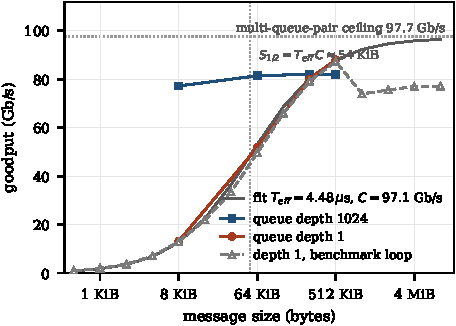
\includegraphics[width=\columnwidth]{figures/msgsize.pdf}
  \caption{Goodput against message size at queue depth 1 and queue depth 1024,
    with Equation~\ref{eq:fixedoffset} fitted to the depth-1 points
    ($T_{\text{eff}} = 4.48$\uS{}, $C = 97.1$\Gbps{}). The depth-1024 arm sits
    on the loss equilibrium of \anom{03} rather than on the ceiling. Data:
    \texttt{RESULTS-p2-msgsize}, \texttt{RESULTS-p4-kernels}.}
  \Description{Log-linear plot of goodput against message size for three arms: a benchmark depth-one loop, a true depth-one engine arm, and a depth-1024 engine arm, with the fixed-offset law fitted to the depth-one points.}
  \label{fig:msgsize}
\end{figure}

The latency floor is 2.10\uS{} median and 2.23\uS{} at the 99th percentile for
a two-byte RDMA write, and 3.99\uS{} for a read, against a measured switch
path of 2.08\uS{}. Against a default TCP socket on the same wire, RDMA is
about $3.5\times$ the bandwidth and about $18\times$ better in latency.

\subsection{The loss equilibrium and the drain window}
\label{sec:meas:drain}

P2 reported a single-queue-pair write and send ``cap'' near 78\Gbps{} that a
second queue pair recovered to the fabric ceiling of 97.7\Gbps{}, and read it
as a requester-side hardware limit. P3 found the number was not constant: send
at 64\,KiB reproduced 78.0\Gbps{} exactly, write at 64\,KiB reached
91.7\Gbps{}, read at 1\,MiB reached 96.7\Gbps{}. P4 resolved it. A single
queue pair sustains 92 to 97\Gbps{} \emph{in burst} at every size. What P2
measured is an equilibrium: a saturated deep pipeline pushes the responder past
its ingress discard threshold, the responder drops at its physical-layer
ingress with no transport signal, and go-back-N recovery costs up to about
16\,\% of goodput. The counter signature is exact and repeatable: the sender
accumulates \ctr{packet\_seq\_err} and \ctr{roce\_adp\_retrans}, the receiver
accumulates \ctr{rx\_discards\_phy}, \ctr{out\_of\_sequence} and a few pause
frames, and \ctr{rx\_out\_of\_buffer} never moves. Depth-one flows and paced
flows are completely clean.

The pacing result is the surprising one. Figure~\ref{fig:drain} shows the gap
sweep. At 8\,KiB, inserting a 4\uS{} inter-burst gap \emph{raises} wall goodput
from 77.5 to 88.2\Gbps{}, a gain of 13.8\,\%, because the gap lets the
responder's ingress drain and removes the retransmission tail entirely. Above
the threshold the duty-cycle model, bytes divided by burst plus gap, is exact
to $\pm 0.1\,\%$; below it, it misses by about 16\,\% at exactly and only the
points where the loss counters move. The threshold is size dependent: at least
4\uS{} at 8\,KiB, and between 4 and 100\uS{} at 64\,KiB, where the 4\uS{}
point still discards about 30\,000 packets per run. Serving decode traffic,
whose per-layer compute gaps run from 4 to 368\uS{}, therefore sits in the
lossless, exactly predictable regime; only back-to-back saturation is lossy.

\begin{figure}[t]
  \centering
  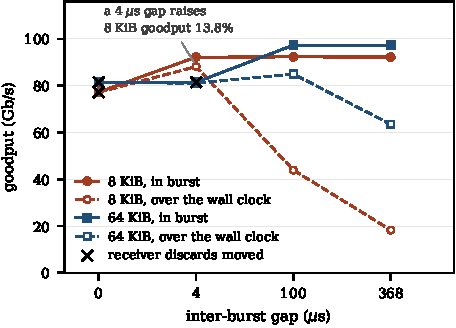
\includegraphics[width=\columnwidth]{figures/drain.pdf}
  \caption{Drain window. Goodput inside a burst and over the wall clock against
    inter-burst gap, at 8\,KiB and 64\,KiB. Points where the receiver's
    \ctr{rx\_discards\_phy} moved are marked. Above the size-dependent
    threshold the duty-cycle model is exact; at 8\,KiB a 4\uS{} gap raises
    wall goodput by 13.8\,\%. Data: \texttt{RESULTS-p4-kernels}.}
  \Description{Line plot of goodput inside a burst and over the wall clock against the inter-burst gap at 8 KiB and 64 KiB, with the points at which the receiver ingress discard counter moved marked.}
  \label{fig:drain}
\end{figure}

Two further asymmetries fall out of the same mechanism. Full duplex is
\emph{cleaner} than one direction: at 91.8\Gbps{} per direction no counter
moves, while a single direction at 93.4\Gbps{} drops, so the responder's
discard threshold sits between the two. And the full-duplex aggregate is
195.0\Gbps{}, which is 99.8\,\% of twice the 97.7\Gbps{} ceiling, with zero
counter movement, at up to 320 queue pairs per direction. The 180\Gbps{} that
P2 reported for the same configuration is an artifact of the benchmark's
bidirectional mode.

\subsection{The internal budget}

Driving loopback traffic and wire traffic into one adapter at once caps total
ingress near 197\Gbps{}, and the split is not fair: the wire flow keeps 99 to
99.8\,\% of its solo rate and the loopback flow absorbs the entire shortfall,
falling to about 51\,\%. The registered hypothesis had been PCIe pressure, and
it is wrong: \ctr{outbound\_pci\_stalled\_rd} and
\ctr{outbound\_pci\_stalled\_wr} were exactly zero at every point of the entire
campaign, including 195\Gbps{} of host-loopback traffic at 4\,MiB across 64
queue pairs. PCIe Gen4 is never the bottleneck at 100\,GbE. What binds is an
internal processing budget with a fixed priority order, and colocated ranks
exchanging over adapter loopback starve under wire load.

\subsection{Congestion control that nobody configured}
\label{sec:meas:cc}

This is the finding the campaign revised most often, and the sequence is worth
stating because the final answer contradicts both the site's belief and our own
two intermediate inferences.

P2 concluded that the fabric never marks ECN, on the evidence that
\ctr{np\_ecn\_marked\_roce\_packets} was zero across 2.5\,TB and $1.09 \times
10^{9}$ packets. P3 corrected that: the same runs moved \ctr{np\_cnp\_sent} and
\ctr{rp\_cnp\_handled} in nearly every phase, so DCQCN was plainly active and
the marking counter is simply inert on these firmware revisions
(\anom{07}). Since a notification point emits a CNP only on receipt of a
CE-marked packet, we inferred that the switch marks. P5a and an endpoint
configuration audit repeated that inference with more evidence: under a
two-to-one incast the receiver emitted 78\,058 CNPs and the senders handled
179\,746, with \ctr{rp\_cnp\_ignored} exactly zero, which proves both a
notification point and a reacting reaction point at firmware default.

P6 refuted the inference at its root. With per-packet logging of $6.7 \times
10^{8}$ packets, at two distinct differentiated-services classes, with the
switch's egress buffer full and dropping 6.36\,\% of traffic, and with 100\,\%
of arriving packets carrying ECT(0) and therefore markable, the number of
CE-marked packets observed was \emph{zero}. The switch does not mark. It
tail-drops, and $K_{\min}$, $K_{\max}$ and $P_{\max}$ are undefined for it.
What generates the notifications is the receiving adapter, from its own ingress
congestion: the receiver's \ctr{np\_cnp\_sent} rises from 38 per second at
idle to 2262 per second exactly during reliable fan-in, which is 283 CNPs per
second per congested queue pair, or one per 3.54\mS{} (\anom{16}). The site's
belief that ECN was off was right about the switch and wrong about the
consequence; our own two intermediate readings were wrong about the marking
point.

A separate probe explains why the traffic was markable in the first place.
P5b requested a Not-ECT control by setting the type-of-service byte to zero and
found the treatment never reached the wire. A standalone probe that reads the
real inbound IP header shows that the adapter overwrites the two ECN bits to
ECT(0) on every RoCEv2 transmit while honouring the differentiated-services
field exactly (\anom{06}):

\begin{center}\small
\begin{tabular}{@{}llll@{}}
  \toprule
  requested & meaning & on the wire & \\
  \midrule
  105 & DSCP 26 $+$ ECT(1)   & 106 & DSCP 26 $+$ ECT(0) \\
  104 & DSCP 26 $+$ Not-ECT  & 106 & DSCP 26 $+$ ECT(0) \\
  0   & DSCP 0 $+$ Not-ECT   & 2   & DSCP 0 $+$ ECT(0) \\
  2   & DSCP 0 $+$ ECT(0)    & 2   & unchanged \\
  \bottomrule
\end{tabular}
\end{center}

Not-ECT RoCE cannot be produced from verbs on this adapter. The practical
consequence is that a default collective job, which sets no type of service at
all, is exactly as ECN-capable and as DCQCN-controlled as our instrumented
traffic, so the congestion behaviour measured here is a property of the
deployment rather than of the harness.

The reaction dynamics are slow. Under a two-to-one incast the first rate cut of
at least 30\,\% arrives after 3, 16 and 39\mS{} in three repeats, fair share is
reached after 5\mS{}, 1.8\,s and 2.3\,s, and recovery to at least 95\,\% of the
solo rate takes $447 \pm 10$\mS{}. The increase is additive at about 0.107
falling to 0.093\Gbps{} per millisecond. The steady two-flow split is 50.18 and
50.13\Gbps{} on a 99.30\Gbps{} wire. Compared with the algorithm's published
defaults the reaction is 2 to 20 times slower and the recovery about
$4.5\times$ slower (\anom{18}), so any study that needs the transient must
carry these numbers and not the defaults.

\subsection{Incast is a tax, not a collapse}

Two senders into one receiver at 1\,MiB messages fill the wire, 99.39\Gbps{}
received, and deliver 73.89\Gbps{} of application goodput. The missing
26.9\,\% of the link is retransmission. The fabric drops 1.65\,\% of packets,
and because each loss forces go-back-N recovery, that 1.65\,\% amplifies about
$16\times$ into the goodput deficit (\anom{11}). Two independent accountings,
the receiver's \ctr{rx\_write\_requests} counter multiplied by message size and
the senders' own completion accounting, agree to 0.02\,\%. The identity is
\begin{equation}
  B_{\text{app}} \;=\; B_{\text{wire}} \cdot
    \bigl(1 - p_{\text{loss}} \cdot A_{\text{gbn}}\bigr),
  \label{eq:incasttax}
\end{equation}
with DCQCN holding $p_{\text{loss}}$ near $10^{-3}$ and $A_{\text{gbn}}$ the
go-back-N amplification factor, measured at about 16 here. That number is worth
a second look: the whole message is 256 packets at this maximum transmission
unit, so retransmitting an entire message on every loss would give
$A_{\text{gbn}} = 256$ and a goodput of zero. The measured 16 says the unit
that is actually replayed is the requester's outstanding window, about 64\,KiB,
and not the message. $A_{\text{gbn}}$ is therefore \evcal{}: it is bounded above
by $S_{\text{msg}}/S_{\text{pkt}}$, it grows with message size, and its value
is a property of a window whose size the specification does not fix.

Fair share is excellent, 50.4 against 49.6, with a four-hertz standard deviation of 0.26\Gbps{} and no
starvation. Fan-out is free: one sender to two receivers delivers 97.83\Gbps{}
split 50.000 to 50.000 with zero counter movement. Only fan-in pays.

At small messages there is no incast penalty at all. A single sender reaches
16.7 million 512-byte messages per second, and the two-sender aggregate reaches
20.5 million, which is 23\,\% \emph{above} the best single sender: at that size
the system is bound by the sender's message rate, not by the receiver or the
wire. Unreliable datagrams under the same two-to-one overload deliver exactly
$0.500 \pm 0.000$ of the offered load with zero movement on every watched
counter at all three nodes (\anom{12}), which is the lossy fabric in one
number.

\subsection{The fabric under the endpoint}
\label{sec:meas:fabric}

P6 calibrated the fabric from the endpoints, because no switch counters were
available. The four nodes share one non-blocking leaf: the latency matrix over
all six pairs spans 1.98 to 2.11\uS{}, a range of 0.13\uS{}, which is smaller
than the repeat-to-repeat spread within one direction and far below the
0.6 to 2.0\uS{} that one extra hop would add; sixteen fresh five-tuples are
unimodal within 0.10\uS{}, so there is one path and no measurable equal-cost
multipath from these nodes; a ring of four runs at 391.94\Gbps{} with every
port at 97.98\Gbps{}.

The per-port egress buffer is a tail-drop queue of about 5.2\,MB.
Figure~\ref{fig:incast} (bottom) shows the identity that measures it: two paced senders
step from below to above the port rate, and the product of the excess rate and
the time from the start of queue build to the first sustained loss is constant
at 5.04 to 5.39\,MB across excess rates of 4.8, 9.7 and 19.7\Gbps{}, a spread
of 6.8\,\%. An independent estimate from the post-overload drain tail gives
$5.76 \pm 2.45$\,MB. The drain rate is 99.995\Gbps{} in all twelve runs, and
loss in steady overflow equals the excess rate to better than 0.04\Gbps{}.
The buffer is \evinf{}: it is measured entirely through its victims.

\begin{figure}[t]
  \centering
  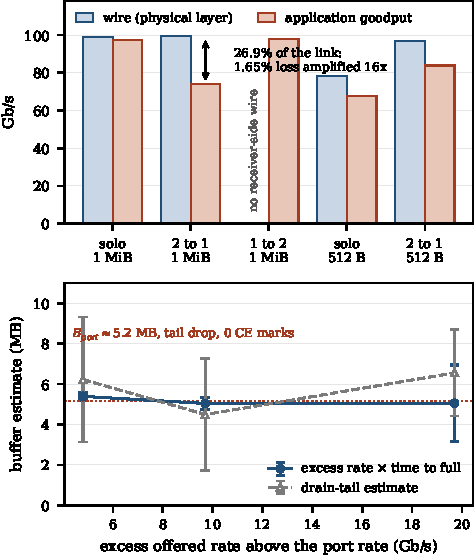
\includegraphics[width=\columnwidth]{figures/incast.pdf}
  \caption{Top: the incast tax. Physical-layer receive rate against
    application goodput for the two-to-one cases and their solo and fan-out
    controls. The wire stays full and the deficit is retransmission. Bottom:
    the switch buffer identity. Excess rate times time to buffer-full is
    constant across three excess rates, giving a tail-drop egress buffer of
    about 5.2\,MB; the independent drain-tail estimate is shown beside it, and
    the fraction of packets marked congestion-experienced is zero at every
    point. Data: \texttt{RESULTS-p5a-incast}, \texttt{RESULTS-p6-fabric}.}
  \Description{Two stacked panels. The top panel is a grouped bar chart of physical-layer wire rate against application goodput for five incast and control cases. The bottom panel plots two independent switch buffer estimates against the excess offered rate.}
  \label{fig:incast}
\end{figure}

There is no link-level flow control anywhere in the path. Priority flow control
is off in the hardware register on every node; the adapters do emit 802.3x
global pause under load, on the order of 760 frames per run, and
\ctr{rx\_pause\_ctrl\_phy} is zero at every node in every phase of the entire
campaign. The pause loop is one hop long, receiver to switch, and terminates
there (\anom{08}).

Finally, a lone reliable flow above about 94\Gbps{} loses $0.1798\,\% \pm
0.0012$ of its packets at the receiver's physical-layer ingress, over eight
repeats and 32 fresh five-tuples, unimodal and path independent. The loss is
bursty: about 73 packets, roughly 94\uS{}, per event. At least 10\Gbps{} of
reverse traffic cuts the event count by $12.5\times$ without changing the burst
length, 1\Gbps{} of reverse traffic does nothing, and receiver CPU load does
nothing. \ctr{rx\_out\_of\_buffer} is zero in every run, so this is not receive
queue exhaustion. This is \anom{17}, and no block in the model reproduces its
mechanism yet.

\subsection{Counters do not mean what they say}

Any tool that detects RDMA anomalies from counters has to know four things
about this hardware (\anom{19}, \anom{09}, \anom{07}).
\ctr{packet\_seq\_err} counts loss \emph{bursts}, not lost packets: under a
lone flow the receiver discarded 107\,542 packets while the sender recorded
1\,465 sequence errors, a ratio of about 73, because go-back-N collapses one
contiguous drop burst into one sequence error. \ctr{rx\_discards\_phy} counts
adapter-ingress loss exactly, and switch-side loss appears in neither counter.
\ctr{rx\_out\_of\_buffer} never moves, in any phase, because receive queues
were always posted deep and RDMA writes consume none. \ctr{rx\_write\_requests}
is an exact application-goodput counter, agreeing with engine accounting to
0.01\,\%, but it is 32 bits wide and wraps at high message rates.
\ctr{np\_ecn\_marked\_roce\_packets} is inert. Firmware 16.31 counts
\ctr{local\_ack\_timeout\_err} where firmware 16.32 counts zero for identical
behaviour. And senders handle $2.24\times$ the CNPs the receiver reports
sending, reproducibly, which we record and do not explain.

\subsection{Corrected attributions}

Three widely quoted numbers from this campaign are wrong as originally
attributed, and the corrections are part of the result.

The 78\Gbps{} single-queue-pair ``cap'' is a loss and retransmission
equilibrium of a saturated deep pipeline on a fabric without flow control, not
a requester limit; in burst the same queue pair reaches 92 to 97\Gbps{}.

The 3.07 million packets per second single-queue-pair unreliable-datagram
receive cap, along with a spectacular 47.5\,\% silent discard, belonged to the
measurement engine's receive path and not to the adapter. On the wire, with the
per-packet logger instead of the engine, one receive queue pair absorbs 5.51
million 2\,KiB packets per second and 2.98 million 4\,KiB packets per second
with only the 0.17 to 0.19\,\% ingress floor, and four queue pairs are slightly
worse. The row survives in the anomaly table with kind \textit{tool}
(\anom{01}), reproduced by nothing, because deleting it would erase the reason
several downstream numbers changed.

The 129\Gbps{} unreliable-datagram ceiling measured on host loopback is
packets-per-second bound and does not transfer: on the wire the same transport
is bandwidth bound and clean at 99.4\Gbps{}.

\subsection{The anomaly table}

Table~\ref{tab:anomaly} is the campaign's output in the form the architecture
consumes. Each row names a trigger, an effect with a magnitude, an evidence
phase, and a \emph{kind} that says how the model is required to reproduce it:
\textit{emergent} from a named mechanism and validated against a band,
\textit{injected} by rule because the mechanism is not public,
\textit{fabric} because it belongs to the switch or the link, \textit{counter}
because it is a facade behaviour with no datapath effect, or \textit{tool}
because it is an artifact of the instrument. The table is data, not prose: it
is a constant array in the model's sources with a generated projection that a
test compares byte for byte, and one test per row asserts the effect inside its
registered band.

\begin{table*}[t]
  \centering
  \footnotesize
  \setlength{\tabcolsep}{3.5pt}
  \renewcommand{\arraystretch}{1.12}
  \caption{The nineteen-row anomaly table: the verification contract between
    the measurements and the architecture. \textit{Kind} states how the model
    is required to reproduce the row. The block column names the block of
    \S\ref{sec:arch} that owns it. Rows \anom{01} and \anom{16} through
    \anom{19} are post-specified corrections made after the phase that owns
    them was frozen, and are labelled as such in the campaign records.}
  \label{tab:anomaly}
  \newcolumntype{R}[1]{>{\raggedright\arraybackslash}p{#1\textwidth}}
  \begin{tabular}{@{}l R{0.115} R{0.185} R{0.30} R{0.065} l l@{}}
    \toprule
    Id & Anomaly & Trigger & Effect and magnitude & Kind & Block & Evidence \\
    \midrule

    \anom{01} & UD receive cap &
    one UD queue pair receiving above 3.07\,Mpps through the measurement engine &
    re-attributed: the knee and the 47.5\,\% silent loss were the engine's
    receive path. On the wire one UD queue pair absorbs 5.51\,Mpps of 2\,KiB
    with only the 0.17 to 0.19\,\% ingress floor &
    tool & none & P3, P6 \\

    \anom{02} & two-SGE send sequence-error storm &
    RC send with two gather entries of 512\,B each, 32 queue pairs &
    \ctr{packet\_seq\_err} of 68\,k to 400\,k per 30\,s; the one-entry control
    at identical bytes is exactly zero; goodput within 3\,\% &
    injected & B7, B8 & P3 \\

    \anom{03} & saturated loss equilibrium &
    one RC queue pair, queue depth 1024, no inter-burst gap, above about
    92\Gbps{} &
    responder ingress discards plus a go-back-N tail; goodput settles at 78 to
    92\Gbps{} &
    emergent & B10 & P2, P3, P4 \\

    \anom{04} & drain window &
    inter-burst gap of at least 4\uS{} at 8\,KiB, 4 to 100\uS{} at 64\,KiB &
    discards go to zero; goodput follows the duty model within 0.1\,\%; a
    4\uS{} gap raises 8\,KiB goodput by 13.8\,\% &
    emergent & B10 & P4 \\

    \anom{05} & loopback starvation &
    loopback and wire ingress together above 197\Gbps{} &
    wire keeps 99\,\%, loopback drops to 51\,\%, no PCIe stall &
    emergent & B17 & P3 \\

    \anom{06} & ECT(0) stamping &
    any RoCEv2 transmit &
    ECN bits forced to ECT(0) regardless of requested type of service; DSCP
    honoured &
    injected & B7 & P5b \\

    \anom{07} & inert marking counter &
    any traffic &
    \ctr{np\_ecn\_marked\_roce\_packets} stays zero while CNPs are generated &
    counter & B19 & P3, P5a, P5b \\

    \anom{08} & one-hop pause &
    receiver overload &
    receiver emits global pause; no peer ever receives one &
    fabric & B9 $+$ fabric & P3, audit \\

    \anom{09} & firmware counter variant &
    retransmission &
    firmware 16.31 counts \ctr{local\_ack\_timeout\_err}; firmware 16.32
    counts zero &
    counter & B19 & P5a \\

    \anom{10} & duplex cleaner than simplex &
    full duplex at 91.8\Gbps{} per direction against one direction at
    93.4\Gbps{} &
    duplex counter-clean, simplex dirty; the discard threshold sits between &
    emergent & B10 & P4 \\

    \anom{11} & incast amplification &
    $N$ senders into one receiver, 1\,MiB messages &
    wire full; goodput tax equals loss rate times a go-back-N amplification
    factor ($16\times$ at 1.65\,\% loss, a 26.9\,\% tax) &
    emergent & B7, B13 & P5a \\

    \anom{12} & UD one-over-$N$ delivery &
    $N$ UD senders into one receiver &
    delivery exactly $1/N$; no endpoint counter moves &
    fabric & fabric & P5a \\

    \anom{13} & MTU tax &
    path MTU 1024 against 4096 &
    5.6\,\% of goodput &
    emergent & B7 & P2 \\

    \anom{14} & host-bound message rate &
    small messages, single process &
    3.87\,Mpps on one queue pair at 1\,KiB; 16.7\,Mmsg/s per sender at 512\,B &
    emergent & B6 & P2, P5a \\

    \anom{15} & memory-region insensitivity &
    12\,000 memory regions; 1024 regions of 64\,KiB; gathers except \anom{02} &
    no throughput effect &
    emergent by absence & B5 & P3 \\

    \anom{16} & endpoint-generated notification &
    RC fan-in on a fabric whose switch never marks &
    the receiver signals its own ingress congestion: \ctr{np\_cnp\_sent} rises
    from 38 to 2262 per second, which is 283 CNP/s per congested queue pair &
    emergent & B14 & P6 \\

    \anom{17} & ingress stall bursts &
    one lone RC flow above about 94\Gbps{} &
    0.18\,\% of packets lost at the receiver's ingress in bursts of about 73
    packets (94\uS{}), path independent over 32 five-tuples; 10\Gbps{} of
    reverse traffic cuts the event count $12.5\times$ without changing the
    burst length &
    emergent & B10 & P6 \\

    \anom{18} & slow DCQCN dynamics &
    a reaction point under two-to-one RC fan-in &
    cut of at least 30\,\% after 3 to 39\mS{}; fair share after 5\mS{} to
    2.3\,s; recovery to 95\,\% in $447 \pm 10$\mS{}; additive increase about
    0.1\Gbps{} per millisecond &
    emergent & B15 & P6 \\

    \anom{19} & counter semantics under loss &
    any loss on the path &
    \ctr{packet\_seq\_err} counts loss bursts, $73\times$ fewer than packets
    lost; \ctr{rx\_discards\_phy} is exact; switch loss appears in neither;
    \ctr{out\_of\_buffer} never moves; senders handle $2.24\times$ the CNPs the
    receiver reports sending &
    counter & B19 & P6 \\

    \bottomrule
  \end{tabular}
\end{table*}


\section{Block architecture}
\label{sec:arch}

This section is the paper's main artifact. It defines an RDMA endpoint in
nineteen blocks, targeting an AMD Alveo U55C accelerator card first and
expandable to an application-specific implementation, such that every block
names the measured behaviour it is required to reproduce, the evidence class of
every parameter it carries, the block of the golden C model it corresponds to,
and the control and status registers it publishes.

\subsection{Target}
\label{sec:arch:target}

The first target is one Alveo U55C card~\cite{alveo-u55c}.
Table~\ref{tab:u55c} lists the resources the architecture depends on. The choice is deliberate rather than
convenient: the card carries two 100\,GbE-capable cages and the integrated
Ethernet hard blocks to drive them, which is exactly the port count the
measured device has; it carries high-bandwidth memory large enough that
queue-pair context and memory translation need not be host resident at the
scale we care about; and its PCIe attachment is the same generation as the
measured host, so a comparison against measured host-side behaviour is not
confounded by the link.

\begin{table}[t]
  \centering
  \small
  \caption{Alveo U55C resources the architecture depends on.
    \TODO{confirm every row against the current data sheet before submission;
    the numbers below are the ones the design was sized against.}}
  \label{tab:u55c}
  \begin{tabular}{@{}ll@{}}
    \toprule
    Resource & Figure used for sizing \\
    \midrule
    Logic & about 1.30\,M lookup tables, 2.6\,M registers \\
    On-chip memory & about 70\,Mb block RAM, 270\,Mb ultra RAM \\
    Device memory & 16\,GB HBM2, about 460\,GB/s aggregate \\
    Network & 2 QSFP28 cages, 2 integrated 100\,GbE MAC cores \\
    Host & PCIe Gen3 $\times 16$, or Gen4 $\times 8$ \\
    \bottomrule
  \end{tabular}
\end{table}

Every dimension that a different target would change is a parameter, listed in
\S\ref{sec:arch:expand}: link rate, path maximum transmission unit, queue-pair
count, memory-region count, buffer sizes and port count. The application-specific
path replaces high-bandwidth memory with on-die static RAM and replaces the
soft interconnect adapters with hard macros, and keeps the same
register-transfer-level sources and the same register map.

\subsection{Two interconnects}
\label{sec:arch:interconnect}

The architecture separates moving data from observing the machine, and gives
each its own interconnect.

\textbf{The AXI4 data path} carries everything with a byte count: host-memory
reads for work-queue elements, context, translations and payload; host-memory
writes for placed payload and completion-queue entries; and high-bandwidth
memory traffic for context, translation and buffer backing. It is a
512-bit AXI4 fabric, which at the Ethernet core clock of 322.266\,MHz supplies
about 165\Gbps{} per direction, comfortably above the 100\Gbps{} line rate and
above the 197\Gbps{} internal budget the measurements found when loopback and
wire traffic share the machine. Read and write channels are independent, and
every initiator carries a transaction identifier that maps to one of the
transaction classes the model already accounts separately: user access region,
doorbell record, work-queue element, context, translation, payload read,
payload write, completion-queue entry, command and interrupt.

\textbf{The AXI4-Lite monitoring network on chip} carries nothing with a byte
count. It is a unidirectional ring of register slices, one stop per block, with
a single initiator at the host interface, 32-bit data and a 4\,KiB aperture per
stop. A ring rather than a crossbar because a crossbar with nineteen slaves and
one master is all cost and no benefit here: monitoring traffic is rare, entirely
tolerant of latency, and the ring's one register stage per stop is free timing
closure and a fixed, small resource cost that does not grow quadratically as
blocks are added. The ring is physically and logically separate from the data
path, so reading a counter cannot perturb the datapath timing that the counter
describes, which is the property that makes the resulting traces usable as
verification evidence.

\subsection{The register map}
\label{sec:arch:csr}

Every block occupies one 4\,KiB page of a single versioned map, addressed from
the control base address register. The first sixteen bytes of every page are
identical:

\begin{center}\small
\begin{tabular}{@{}lll@{}}
  \toprule
  Offset & Field & Meaning \\
  \midrule
  \texttt{0x000} & \csr{MAP\_VERSION}   & major and minor of the whole map \\
  \texttt{0x004} & \csr{BLOCK\_ID}      & B1 to B19 \\
  \texttt{0x008} & \csr{BLOCK\_VERSION} & this block's own version \\
  \texttt{0x00C} & \csr{CAPABILITIES}   & optional features present \\
  \bottomrule
\end{tabular}
\end{center}

\noindent
Software that knows \csr{MAP\_VERSION} knows the layout of every page, and a
block that gains a field bumps \csr{BLOCK\_VERSION} without invalidating
readers of the others. Three map-wide mechanisms follow.

\textbf{One clock.} A free-running 64-bit counter, clocked from the reference
the Ethernet subsystem already needs, ticks every 6.4\nS{} at 156.25\,MHz. It is
broadcast to every block, and every timestamped event in the design is stamped
from it. The measured device offers a hardware timestamp on received packets
and nothing else; here every block's events share one time base.

\textbf{Coherent snapshots.} Writing \csr{SNAPSHOT} at the map level asserts a
broadcast strobe that latches every block's counters and occupancies into a
shadow bank together with the current timestamp. The campaign spent real effort
working around the fact that counters on the measured device are read
non-atomically and are cached by the driver for 10\mS{}, which is why rates
below that window are meaningless there. Here a read set is coherent by
construction.

\textbf{Counter width and a compatibility mode.} All counters are 64 bits, which
removes the wrap that makes \ctr{rx\_write\_requests} unusable at high message
rates on the real device. Because fidelity to the real device is sometimes the
point, a \csr{WRAP32\_COMPAT} bit makes the mirrored counters wrap at 32 bits
exactly as the original does, so a tool written against the real adapter can be
tested against this one.

The map has two halves. The \emph{mirror} half carries counters named exactly as
the real device names them, with the real semantics preserved including the ones
that are wrong: \ctr{np\_ecn\_marked\_roce\_packets} is present and stays zero
(\anom{07}), \ctr{packet\_seq\_err} counts loss bursts and not lost packets
(\anom{19}), \ctr{out\_of\_buffer} exists and never moves under the conditions
the campaign covered, and a \csr{FW\_VARIANT} field selects whether
\ctr{local\_ack\_timeout\_err} counts or stays zero (\anom{09}). The
\emph{extension} half carries what the real device does not expose and the FPGA
can: the instantaneous and high-water occupancy of every internal queue, the
credit state of every arbiter, per-stage service counts, and the reaction
point's rate and $\alpha$ per queue pair. \S\ref{sec:verify:fpga} returns to
what that buys.

\begin{figure*}[t]
  \centering
  %% Top-level block architecture.  Pure TikZ, no external assets.
%% Coordinates are in units of 0.9 cm; the picture is sized to the text width
%% of a two-column page and does not depend on the document class.
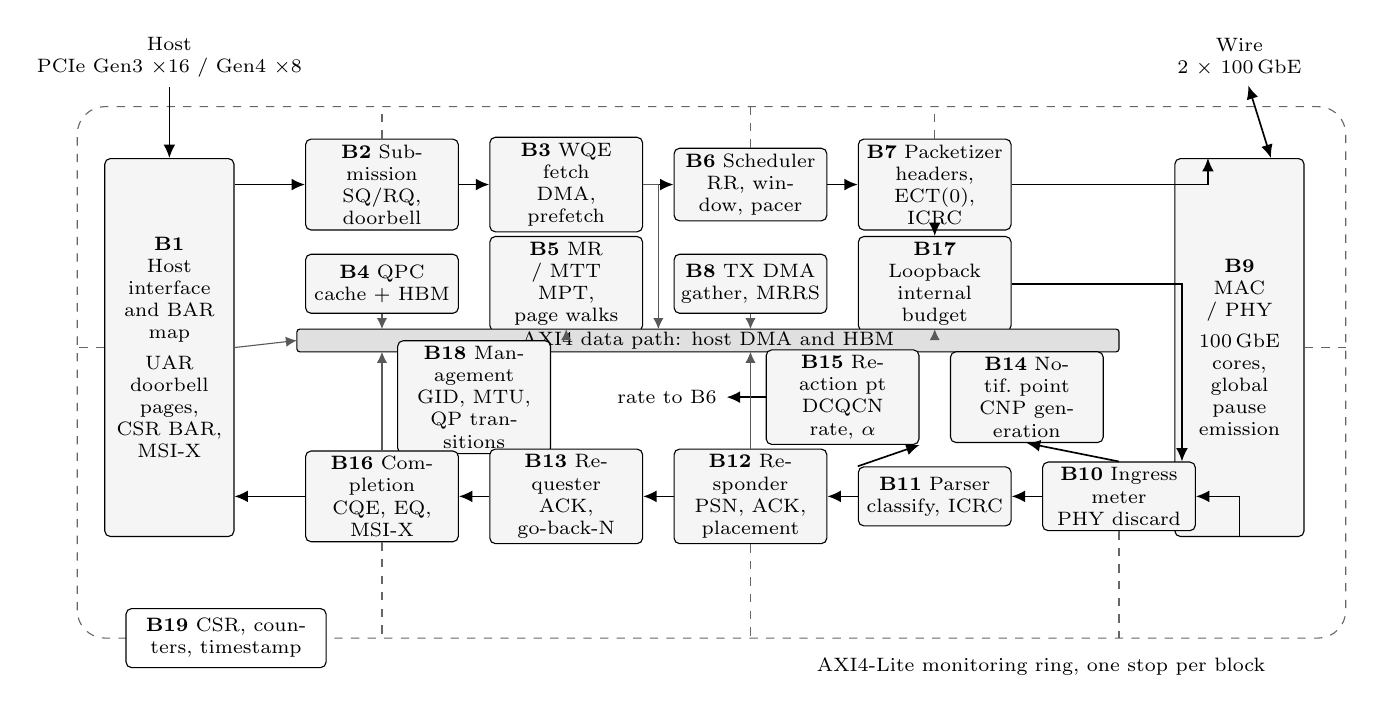
\begin{tikzpicture}[
  x=0.9cm, y=0.9cm,
  font=\scriptsize,
  blk/.style   = {draw, rounded corners=2pt, align=center, fill=black!4,
                  text width=18mm, inner sep=2pt, minimum height=7.5mm},
  tall/.style  = {draw, rounded corners=2pt, align=center, fill=black!4,
                  text width=15mm, inner sep=2pt, minimum height=48mm},
  ext/.style   = {align=center, font=\scriptsize},
  bus/.style   = {draw, fill=black!12, rounded corners=1pt},
  flow/.style  = {-{Latex[length=1.7mm,width=1.5mm]}, semithick},
  duplex/.style= {{Latex[length=1.7mm,width=1.5mm]}-%
                  {Latex[length=1.7mm,width=1.5mm]}, semithick},
  axi/.style   = {-{Latex[length=1.4mm,width=1.3mm]}, thin, draw=black!65},
  mon/.style   = {dashed, draw=black!60, thin},
]

%% ==== monitoring ring, drawn first so blocks sit on top of it =============
\draw[mon, rounded corners=10pt] (0.3,-1.0) rectangle (18.2,6.5);

%% ==== host and wire, outside the ring =====================================
\node[ext] (host) at (1.6,7.2) {Host\\PCIe Gen3 $\times$16 / Gen4 $\times$8};
\node[ext] (wire) at (16.7,7.2) {Wire\\2 $\times$ 100\,GbE};

%% ==== left and right edge blocks ==========================================
\node[tall] (b1) at (1.6,3.1)
  {\textbf{B1}\\Host interface\\and BAR map\\[3pt]UAR doorbell pages,
   CSR BAR, MSI-X};
\node[tall] (b9) at (16.7,3.1)
  {\textbf{B9}\\MAC / PHY\\[3pt]100\,GbE cores, global pause emission};

%% ==== lane 1: transmit datapath ===========================================
\node[blk] (b2)  at (4.6,5.4)  {\textbf{B2} Submission\\SQ/RQ, doorbell};
\node[blk] (b3)  at (7.2,5.4)  {\textbf{B3} WQE fetch\\DMA, prefetch};
\node[blk] (b6)  at (9.8,5.4)  {\textbf{B6} Scheduler\\RR, window, pacer};
\node[blk] (b7)  at (12.4,5.4) {\textbf{B7} Packetizer\\headers, ECT(0),
  ICRC};

%% ==== lane 2: context, translation, gather, loopback ======================
\node[blk] (b4)  at (4.6,4.0)  {\textbf{B4} QPC\\cache $+$ HBM};
\node[blk] (b5)  at (7.2,4.0)  {\textbf{B5} MR / MTT\\MPT, page walks};
\node[blk] (b8)  at (9.8,4.0)  {\textbf{B8} TX DMA\\gather, MRRS};
\node[blk] (b17) at (12.4,4.0) {\textbf{B17} Loopback\\internal budget};

%% ==== the AXI4 data path bus ==============================================
\draw[bus] (3.4,3.04) rectangle (15.0,3.36);
\node[font=\scriptsize] at (9.2,3.2) {AXI4 data path: host DMA and HBM};

%% ==== lane 3: management and congestion control ===========================
\node[blk] (b18) at (5.9,2.4)  {\textbf{B18} Management\\GID, MTU, QP
  transitions};
\node[blk] (b15) at (11.1,2.4) {\textbf{B15} Reaction pt\\DCQCN rate,
  $\alpha$};
\node[blk] (b14) at (13.7,2.4) {\textbf{B14} Notif.\ point\\CNP generation};

%% ==== lane 4: receive datapath ============================================
\node[blk] (b16) at (4.6,1.0)  {\textbf{B16} Completion\\CQE, EQ, MSI-X};
\node[blk] (b13) at (7.2,1.0)  {\textbf{B13} Requester\\ACK, go-back-N};
\node[blk] (b12) at (9.8,1.0)  {\textbf{B12} Responder\\PSN, ACK, placement};
\node[blk] (b11) at (12.4,1.0) {\textbf{B11} Parser\\classify, ICRC};
\node[blk] (b10) at (15.0,1.0) {\textbf{B10} Ingress meter\\PHY discard};

%% ==== transmit flow =======================================================
\draw[flow] (host) -- (b1.north);
\draw[flow] (b1.east|-b2.west) -- (b2.west);
\draw[flow] (b2) -- (b3);
\draw[flow] (b3) -- (b6);
\draw[flow] (b6) -- (b7);
\draw[flow] (b7.east) -| ([xshift=-4mm]b9.north);
\draw[duplex] ([xshift=4mm]b9.north) -- (wire);

%% ==== receive flow ========================================================
\draw[flow] (b9.south) |- (b10.east);
\draw[flow] (b10) -- (b11);
\draw[flow] (b11) -- (b12);
\draw[flow] (b12) -- (b13);
\draw[flow] (b13) -- (b16);
\draw[flow] (b16.west) -- (b1.east|-b16.west);

%% ==== loopback and the shared ingress budget ==============================
\draw[flow] (b7.south) -- (b17.north);
\draw[flow] (b17.east) -| ([xshift=8mm]b10.north);

%% ==== congestion control ==================================================
\draw[flow] (b10.north) -- (b14.south);
\draw[flow] (b11.north west) -- (b15.south east);
\draw[flow] (b15.west) -- ++(-0.55,0)
  node[left, font=\scriptsize] {rate to B6};

%% ==== AXI4 data path attachments ==========================================
\draw[axi] (b1.east) -- (3.4,3.2);
\draw[axi] (b4.south)  -- (4.6,3.36);
\draw[axi] (b5.south)  -- (7.2,3.36);
\draw[axi] (b8.south)  -- (9.8,3.36);
\draw[axi] (b17.south) -- (12.4,3.36);
\draw[axi] (b16.north) -- (4.6,3.04);
\draw[axi] (b12.north) -- (9.8,3.04);
\draw[axi] (b3.east) -- (8.5,5.4) -- (8.5,3.36);

%% ==== the monitoring ring endpoints =======================================
\draw[mon] (b1.west)  -- (0.3,3.1);
\draw[mon] (b9.east)  -- (18.2,3.1);
\draw[mon] (b2.north) -- (4.6,6.5);
\draw[mon] (b6.north) -- (9.8,6.5);
\draw[mon] (b7.north) -- (12.4,6.5);
\draw[mon] (b16.south) -- (4.6,-1.0);
\draw[mon] (b12.south) -- (9.8,-1.0);
\draw[mon] (b10.south) -- (15.0,-1.0);
\node[blk, fill=white, text width=24mm] (b19) at (2.4,-1.0)
  {\textbf{B19} CSR, counters, timestamp};
\node[font=\scriptsize, anchor=west] at (10.6,-1.4)
  {AXI4-Lite monitoring ring, one stop per block};

\end{tikzpicture}

  \caption{Top-level block architecture. Solid arrows are the AXI4 data path
    and the packet path; the dashed ring is the AXI4-Lite monitoring network on
    chip, which reaches every block and is the only path by which state leaves
    the design for observation. Blocks are numbered as in
    \S\ref{sec:arch:blocks} and in the block column of
    Table~\ref{tab:anomaly}.}
  \Description{Top-level block diagram of the RDMA endpoint: a transmit lane, a context and translation lane, an AXI4 data path bus, a congestion-control lane and a receive lane, between a host interface on the left and a media access block on the right, all enclosed by a dashed AXI4-Lite monitoring ring.}
  \label{fig:arch}
\end{figure*}

\subsection{The blocks}
\label{sec:arch:blocks}

Each block below states, in order: what it does, the state it owns, its
interfaces, the measured behaviour it is required to reproduce with the finding
and anomaly row that pin it, the corresponding block of the golden C model, and
the registers it publishes on the monitoring ring. Register names written as
\ctr{this} are mirrors of names the real device uses; names written as
\csr{THIS} belong to this design.

\subsubsection{B1: Host interface and BAR map}

\textbf{Function.} Terminate the PCIe link and split its traffic in two. Base
address register 0 is the control region: it decodes into the AXI4-Lite
monitoring ring and is the only initiator on it. Base address registers 2 and 4
expose user access region pages, one page per doorbell context, mapped
write-combining into user processes; a store to such a page is a doorbell, and
a store of a full work-queue element to such a page is the inline publication
path that lets the device skip the fetch entirely. The block also owns the
MSI-X table and the pending-bit array, and converts posted writes, non-posted
reads and completions into AXI4 transactions tagged with the class they belong
to.

\textbf{State.} Base-address decode; the user-access-region page ownership map;
write-combining coalescing buffers; the MSI-X table and pending bits;
outstanding read tags and the completion reservation for them.

\textbf{Interfaces.} PCIe Gen3 $\times 16$ or Gen4 $\times 8$ toward the host;
AXI4 master and slave toward the data path; AXI4-Lite master onto the
monitoring ring; a doorbell stream to B2.

\textbf{Must reproduce.} That PCIe is not the bottleneck at 100\,GbE. The
campaign's stall counters were exactly zero at every one of more than 700
points, including 195\Gbps{} of host-loopback traffic at 4\,MiB messages across
64 queue pairs, and including the 197\Gbps{} internal-budget point. The block
must therefore expose \ctr{outbound\_pci\_stalled\_rd} and
\ctr{outbound\_pci\_stalled\_wr} and they must be capable of moving, so that a
later study at a higher rate can show when the link does bind; a model in which
they are hard-wired to zero would be unfalsifiable.

\textbf{Evidence.} The base-address layout, the user-access-region semantics and
the doorbell record are \evdoc{}. Write-combining behaviour and the inline
publication path are \evdrv{} from the provider source. Maximum payload size,
maximum read request size, read-completion-boundary policy and credit pools are
\evdoc{}. The service latencies of each transaction class are \evcal{}.

\textbf{Golden model.} The transaction-level PCIe fabric with its per-class
inventory (user access region, BlueFlame, doorbell record, work-queue element,
context, translation, payload read, payload write, completion-queue entry,
command, interrupt) and the work-queue PCIe binding.

{\raggedright
\textbf{Registers.} \csr{PCI\_LINK\_GEN}, \csr{PCI\_LINK\_WIDTH}, \csr{MPS},
\csr{MRRS}, \ctr{outbound\_pci\_stalled\_rd},
\ctr{outbound\_pci\_stalled\_wr}, \csr{UAR\_WRITES},
\csr{INLINE\_PUBLICATIONS}, \csr{DB\_RECORD\_READS}, and, in the extension
half, \csr{READ\_TAG\_OCCUPANCY} and \csr{WC\_BUFFER\_FLUSHES}.\par}

\subsubsection{B2: Submission engine}

\textbf{Function.} Own the send and receive queue rings. On a doorbell, read the
doorbell record, compute the accepted prefix of newly posted work-queue
elements, and hand their indices to B3 as one batch. Handle inline data, which
arrives with the doorbell rather than through a fetch. Retire slots when B16
says a completion has made them reclaimable.

\textbf{State.} Per queue pair: ring base address and logarithmic size, the
producer index last read from the doorbell record, the device's own consumer
index, the accepted-prefix pointer, and an inline staging buffer.

\textbf{Interfaces.} Doorbell stream from B1; AXI4 read for doorbell records;
work-queue-element index batches to B3; reclaim notifications from B16.

\textbf{Must reproduce.} Accepted-prefix semantics: a single doorbell publishes
an arbitrary prefix of posted work, so the number of memory-mapped writes per
work request falls with the posting batch. The measured consequence is that
posting batch is nearly free: batches of 1 and 64 differ by only $1.16\times$,
because both arms pipeline at the same queue depth. The default send-queue
depth of 1024 must be a parameter and not an assumption, because the campaign's
single most expensive analysis error was reading a tool flag that sets work
requests per posting call as if it set queue depth.

\textbf{Evidence.} Ring geometry, doorbell records and inline semantics are
\evdoc{} and \evdrv{}. The depth default is \evdrv{}. The $1.16\times$ batching
figure is a measured property of the pipeline, and belongs to B6.

\textbf{Golden model.} The submission model and the work-queue core's
accepted-prefix posting with explicit doorbell batches.

{\raggedright
\textbf{Registers.} \csr{SQ\_DEPTH}, \csr{RQ\_DEPTH}, \csr{DOORBELLS\_SEEN},
\csr{WQES\_ACCEPTED}, \csr{INLINE\_BYTES}; extension half
\csr{ACCEPTED\_PREFIX\_HIST}, \csr{SQ\_OCCUPANCY},
\csr{SQ\_OCCUPANCY\_HIGH\_WATER}.\par}

\subsubsection{B3: Work-queue-element fetch}

\textbf{Function.} Read work-queue-element bytes from host memory by direct
memory access, prefetching across a doorbell batch so that the fetch of one
element overlaps the processing of the previous one. Bypassed entirely when the
element arrived inline.

\textbf{State.} Outstanding fetch tags; the prefetch window; a per-queue-pair
fetch cursor; a small reorder buffer, because read completions may return out
of order.

\textbf{Interfaces.} AXI4 read to host memory; decoded work-queue-element
records to B4 and B6.

\textbf{Must reproduce.} One component of the fixed-offset initiation cost
$T_{\text{eff}} = 4.48$\uS{}. The campaign can identify the sum of the
initiation stages and not their split, so the architecture assigns a
parameterised service to each of the five stages (publication, observation,
fetch, context readiness, admission) whose sum is constrained and whose split
is \evcal{}. The block must also not become the depth limiter: with 1024
elements outstanding the machine runs $5.9\times$ faster at 8\,KiB than with
one, so prefetch depth is sized from the outstanding-work window and not the
other way round.

\textbf{Evidence.} The element layout is \evdoc{}; the fetch batching is
\evdrv{}; the stage split of $T_{\text{eff}}$ is \evcal{} and explicitly an
assumption until a work-queue publication campaign lands.

\textbf{Golden model.} The serialized fetch stage of the queue core, backed by
read and completion transactions on the PCIe fabric.

{\raggedright
\textbf{Registers.} \csr{WQE\_FETCH\_BYTES}, \csr{WQE\_FETCH\_COUNT},
\csr{PREFETCH\_DEPTH}; extension half \csr{WQE\_FETCH\_OUTSTANDING},
\csr{WQE\_FETCH\_LATENCY\_HIST}.\par}

\subsubsection{B4: Queue-pair context}

\textbf{Function.} Hold the per-queue-pair state that both the transmit and
receive paths read, in an on-chip cache backed by high-bandwidth memory, and
serve the lookup stage of both paths.

\textbf{State.} Per queue pair: transport type; state in the RESET, INIT, RTR,
RTS, SQD, SQE, ERR machine; send packet sequence number and expected receive
packet sequence number; last acknowledged sequence number; path maximum
transmission unit; destination queue-pair number, global identifier, MAC and
VLAN; traffic class and differentiated-services value; local acknowledgement
timeout and retry counts; the receiver-not-ready timer; the outstanding-work
window; and the congestion-control state, namely the reaction point's $\alpha$,
current rate, target rate, stage, timer and byte counter, and the notification
point's last-CNP timestamp.

\textbf{Interfaces.} AXI4 to high-bandwidth memory for the backing store;
lookup ports to B6 on the transmit side and B11 on the receive side; update
ports from B12, B13 and B15; configuration writes from B18.

\textbf{Must reproduce.} That congestion-control state is persistent per queue
pair and survives across work requests. This is what makes \anom{18} possible:
a rate cut that takes 3 to 39\mS{} to arrive and $447 \pm 10$\mS{} to recover
cannot be modelled by state that resets per message. Path maximum transmission
unit lives here and drives \anom{13}, the 5.6\,\% goodput difference between
1024 and 4096. The state machine's transitions and their legality are
\evdoc{}.

\textbf{Evidence.} Every field is \evdoc{} from the reference manual or the
specification. The cache geometry is \evcal{} with a measured lower bound: 480
active queue pairs against 12\,000 memory regions produced no throughput effect
at all (\anom{15}), so the real device's working set at that scale fits, and
the associativity and replacement policy are not identifiable from outside.

\textbf{Golden model.} The context lookup stage, plus the transport and
congestion-control field groups of the hardware profile.

{\raggedright
\textbf{Registers.} \csr{QP\_COUNT\_ACTIVE}, \csr{QPC\_HITS},
\csr{QPC\_MISSES}, \csr{QP\_SELECT} with a per-queue-pair window exposing
\csr{QP\_STATE}, \csr{QP\_PSN\_SEND}, \csr{QP\_PSN\_EXPECTED} and
\csr{QP\_MTU}; extension half \csr{QPC\_MISS\_SERVICE\_NS},
\csr{QP\_STATE\_HIST}, \csr{QP\_RATE}, \csr{QP\_ALPHA}.\par}

\subsubsection{B5: Memory registration and translation}

\textbf{Function.} Hold the memory protection table (region base, length, keys,
protection domain, access rights) and the memory translation table
(virtual-to-physical mapping), cache both on chip, validate keys and access
rights on every reference, and walk host memory on a miss.

\textbf{State.} Cached protection and translation entries; the page-walk queue;
key and access-right check results.

\textbf{Interfaces.} Lookup ports from B8 (transmit gather) and B12 (receive
placement); AXI4 read for walks; configuration writes from B18.

\textbf{Must reproduce.} \anom{15}, and it is the one row of the table that is
reproduced \emph{by absence}. Twelve thousand memory regions cost $+1.2\,\%$
against a two-region control, and 1024 regions of 64\,KiB were identical to the
control to four significant figures. The architecture therefore sizes the cache
above the measured working set and the block adds no cost in that regime; what
it must \emph{not} do is silently hide a smaller cache, which is why the miss
counters and the service time a miss cost are published separately. The real
device's behaviour beyond the measured working set is unknown and is declared
so.

\textbf{Evidence.} Table layouts, keys and access rights are \evdoc{}; the
cache size is \evcal{} with a lower bound; behaviour past the bound is
\evdecl{}.

\textbf{Golden model.} Not modelled in the current slice, and documented as an
absence rather than assumed to be free; the profile's three-tier context
hierarchy (on-die static RAM, optional device memory, host pinned memory) is
where it lands.

{\raggedright
\textbf{Registers.} \csr{MR\_COUNT}, \csr{MPT\_HITS}, \csr{MPT\_MISSES},
\csr{MTT\_HITS}, \csr{MTT\_MISSES}, \csr{PAGE\_WALKS},
\csr{KEY\_VIOLATIONS}; extension half \csr{XLAT\_CACHE\_OCCUPANCY},
\csr{XLAT\_MISS\_SERVICE\_NS}.\par}

\subsubsection{B6: Scheduler and transmit arbiter}

\textbf{Function.} Choose which queue pair transmits next. Round robin over
queue pairs that are ready, subject to three gates: the per-queue-pair
outstanding-work window, which is released by acknowledgements; the
per-queue-pair and per-device packet-rate and bit-rate limiters; and the
per-queue-pair rate token supplied by the reaction point B15.

\textbf{State.} The ready list and its round-robin pointer; per queue pair the
outstanding bytes and packets and the token bucket; the device-wide token
bucket.

\textbf{Interfaces.} Work-queue-element records from B3; context lookup to B4;
rate from B15; window release from B13; packet-issue grants to B7.

\textbf{Must reproduce.} Four measurements pin this block.
(i)~Queue-depth dominance: 13.2\Gbps{} at depth one against 77.2\Gbps{} at
depth 1024, both at 8\,KiB, a factor of 5.9, which requires a genuine
outstanding-work window rather than one element at a time.
(ii)~\anom{14}, the host-bound message rate: 3.87 million packets per second on
one queue pair at 1\,KiB, and 16.7 million messages per second per sender at
512\,B, which the packet-rate limiters carry.
(iii)~Multi-queue-pair recovery of the ceiling: two or more queue pairs reach
97.7\Gbps{} where one saturating queue pair settles into the loss equilibrium.
(iv)~Skew costs completion time and not bandwidth: with seven queue pairs
carrying different message sizes, the per-queue-pair \emph{message} rate was
identical to three decimal places and the per-queue-pair \emph{byte} rate was
exactly proportional to message size (a spread of 2.000 for a 2:1 size ratio),
with an aggregate of 96.5\Gbps{}. That is precisely the signature of round
robin over message completions, and it is the strongest single piece of
evidence for the arbitration policy in this block.

\textbf{Evidence.} The arbitration policy is \evcal{}, inferred from (iv). The
rate-limiter values are \evcal{}. The existence of a per-queue-pair rate gate
fed by congestion control is \evdoc{} from the algorithm.

\textbf{Golden model.} The scheduler admission stage, the outstanding-work
window and the transmit pacer.

{\raggedright
\textbf{Registers.} \csr{TX\_PPS\_LIMIT}, \csr{TX\_BPS\_LIMIT},
\csr{SCHED\_GRANTS}, \csr{QP\_READY\_COUNT}; extension half
\csr{RR\_POINTER}, \csr{QP\_OUTSTANDING\_BYTES}, \csr{QP\_OUTSTANDING\_PKTS},
\csr{TX\_RATE\_TOKENS}.\par}

\subsubsection{B7: Packetizer and header builder}

\textbf{Function.} Turn a granted message into packets. Segment at the path
maximum transmission unit; allocate packet sequence numbers; build the base
transport header and whichever extended header the operation needs (RETH for
remote address and length, AETH for acknowledgement syndrome and credits, DETH
for the source queue pair of a datagram); wrap the result in the RoCEv2
encapsulation, choosing the UDP source port so that it is stable per queue pair
and spread across queue pairs; write the differentiated-services field through
unchanged and force the two ECN bits to ECT(0); and compute the invariant
cyclic redundancy check.

\textbf{State.} Per queue pair a message cursor and a sequence-number
allocator; header templates cached from the context; the check accumulator.

\textbf{Interfaces.} Grants from B6; context read from B4; payload beats from
B8; packets to B9 for the wire or B17 for loopback.

\textbf{Must reproduce.} \anom{13}, the 5.6\,\% maximum-transmission-unit tax,
which emerges from per-packet header overhead and needs no special rule.
\anom{06}, the ECT(0) stamp, which does not emerge from anything and is
therefore \emph{injected}: the block overwrites the two ECN bits
unconditionally on every RoCEv2 transmit while passing the
differentiated-services field through, exactly as the on-wire probe found. The
number of packets a message becomes here bounds the go-back-N replay of
\anom{11} from above (256 at 1\,MiB), while the measured amplification of
about 16 says the unit actually replayed is the requester's outstanding
window of about 64\,KiB; the incast tax is therefore a downstream consequence
of segmentation, the window and go-back-N, and not a separate rule. Finally
\anom{02}, the sequence-error storm under two-entry gathers, is injected here
as a per-packet drop rule keyed on gather-entry count and size, because the
mechanism is not public and no differential experiment we could run localized
it further than ``the transmit path with two-entry gathers is causal''.

\textbf{Evidence.} Header layouts, the check and the encapsulation are
\evdoc{}. The ECN overwrite is measured, and \evcal{} as to why. The
two-entry-gather rule is \evdecl{} and labelled injected in the table.

\textbf{Golden model.} The packetizer.

{\raggedright
\textbf{Registers.} \ctr{tx\_packets\_phy}, \csr{TX\_PAYLOAD\_BYTES},
\csr{TX\_HEADER\_BYTES}, \csr{PSN\_ALLOCATED}, \csr{ECT0\_STAMPED},
\csr{ICRC\_GENERATED}, \csr{MTU\_IN\_USE}; extension half
\csr{PACKETS\_PER\_MESSAGE\_HIST}.\par}

\subsubsection{B8: Transmit direct memory access}

\textbf{Function.} Fetch payload. Walk the scatter-gather list, translate each
entry through B5, segment reads at the maximum read request size, manage read
credits and tags, and reorder returning completions into the packet order B7
needs. Bypassed for inline data.

\textbf{State.} Per-packet gather cursor; outstanding read tags; the completion
reorder buffer; credit counters.

\textbf{Interfaces.} AXI4 read to host memory and to high-bandwidth memory for
device-resident buffers; translation lookups to B5; payload beats to B7.

\textbf{Must reproduce.} That gather entries are free. Two-entry gathers cost
nothing in throughput (the storm of \anom{02} is a loss effect, with goodput
within 3\,\%), and no gather configuration the campaign tried moved a
throughput number. That the reorder buffer never becomes the limit at
100\,GbE, consistent with the stall counters staying at zero.

\textbf{Evidence.} Maximum payload size, maximum read request size, the
read-completion-boundary policy and the credit pools are \evdoc{}. Reorder
buffer depth is \evcal{}.

\textbf{Golden model.} The payload-read transaction class of the PCIe fabric.

{\raggedright
\textbf{Registers.} \csr{TX\_DMA\_READ\_BYTES}, \csr{TX\_DMA\_READS},
\ctr{outbound\_pci\_stalled\_rd} (mirrored from B1); extension half
\csr{TX\_DMA\_OUTSTANDING}, \csr{REORDER\_OCCUPANCY}, \csr{SGE\_COUNT\_HIST}.\par}

\subsubsection{B9: Media access control and physical layer}

\textbf{Function.} Drive the two 100\,GbE ports through the device's integrated
Ethernet cores, and emit 802.3x global pause frames when B10 asks for them.
Priority flow control is implemented but disabled by default, to match the
deployment that was measured.

\textbf{State.} Link state per port; the pause state machine; the physical-layer
counter set.

\textbf{Interfaces.} Streaming interfaces to B7 and from B10; the optical cages;
a pause request line from B10.

\textbf{Must reproduce.} The endpoint half of \anom{08}. An overloaded receiver
\emph{does} emit global pause, on the order of 760 frames per twenty-second
run, and no endpoint in the entire campaign ever received a pause frame of any
kind: \ctr{rx\_pause\_ctrl\_phy} was exactly zero at every node in every phase.
The design must therefore never assume that backpressure propagates, and must
publish both directions of the pause counters so that a deployment where it
does propagate is distinguishable from one where it does not.

\textbf{Evidence.} \evdoc{} throughout (IEEE 802.3 and its pause annex).

\textbf{Golden model.} The flow-control field group of the hardware profile:
priority flow control disabled, global pause transmission enabled, pause
propagation false.

{\raggedright
\textbf{Registers.} \ctr{rx\_packets\_phy}, \ctr{tx\_packets\_phy},
\ctr{rx\_discards\_phy}, \ctr{tx\_discards\_phy}, \ctr{tx\_pause\_ctrl\_phy},
\ctr{rx\_pause\_ctrl\_phy}, \ctr{tx\_global\_pause},
\ctr{tx\_global\_pause\_duration}, \ctr{tx\_pause\_storm\_warning\_events},
\ctr{rx\_prio0\_bytes}, \ctr{tx\_prio0\_bytes}, \csr{LINK\_SPEED},
\csr{LINK\_UP}.\par}

\subsubsection{B10: Receive ingress meter}

\textbf{Function.} A finite buffer at the receive port, drained at a service
rate, into which every arriving packet is written before it is parsed. Overflow
discards at the physical layer, with no transport signal of any kind: the
sender learns about it only through the retransmission it eventually causes.
The block also raises the pause request that B9 turns into a frame, and the
congestion signal that B14 turns into a notification packet.

\textbf{State.} Occupancy and its high-water mark; the drain-rate token bucket;
the state of the stall process described below.

\textbf{Interfaces.} From B9 (wire) and B17 (loopback); to B11; pause request to
B9; congestion indication to B14.

\textbf{Must reproduce.} More of the campaign than any other block.
\anom{03}: a saturated deep pipeline settles at 78 to 92\Gbps{} of goodput with
the counter signature \ctr{rx\_discards\_phy} and \ctr{out\_of\_sequence} at
the receiver and \ctr{packet\_seq\_err} and \ctr{roce\_adp\_retrans} at the
sender.
\anom{04}: above a size-dependent inter-burst gap (at least 4\uS{} at 8\,KiB,
between 4 and 100\uS{} at 64\,KiB) the discards go to zero and the duty-cycle
model becomes exact to $\pm 0.1\,\%$; a 4\uS{} gap at 8\,KiB raises wall
goodput by 13.8\,\%.
\anom{10}: full duplex at 91.8\Gbps{} per direction is counter-clean while one
direction at 93.4\Gbps{} is not, so the threshold sits between them.
\anom{17}: a lone flow above about 94\Gbps{} loses $0.1798\,\% \pm 0.0012$ of
its packets here, in bursts of about 73 packets lasting about 94\uS{}, path
independent over 32 fresh five-tuples, with the event count falling
$12.5\times$ under at least 10\Gbps{} of reverse traffic while the burst length
does not move, and with \ctr{out\_of\_buffer} at zero throughout, so it is not
receive-queue exhaustion.

\textbf{Open clause.} The discard ledger does not close, and the paper says so
rather than hiding it. At the \anom{03} operating point the campaign counted
only a few thousand physical-layer discards over a thirty-second window, far
too few to explain a twenty-percent goodput deficit by loss alone. The meter
reproduces the equilibrium at a fitted drain rate; it does not explain it.
\anom{17} is the narrowed form of the missing mechanism, and a second anchor
makes the gap explicit: under fan-in the same receiver absorbed 99.39\Gbps{}
while discarding almost nothing, and one drain rate cannot satisfy both
anchors. This is the block with the most \evcal{} content in the architecture,
and the one whose first hardware build is most worth instrumenting, because the
monitoring ring can publish the occupancy trace that the real device cannot.

\textbf{Evidence.} The existence of a port ingress buffer is \evdoc{}; its
depth, its drain rate and the stall process are \evcal{}, and the stall process
is currently unmodelled.

\textbf{Golden model.} The ingress meter.

{\raggedright
\textbf{Registers.} \ctr{rx\_discards\_phy} (mirror), \ctr{out\_of\_buffer}
(mirror, inert), \csr{INGRESS\_DRAIN\_BPS}, \csr{INGRESS\_DEPTH\_BYTES},
\csr{STALL\_EVENTS}; extension half \csr{INGRESS\_OCCUPANCY},
\csr{INGRESS\_HIGH\_WATER}, \csr{STALL\_BURST\_LEN\_HIST},
\csr{PAUSE\_REQUESTS}.\par}

\subsubsection{B11: Receive parser and classifier}

\textbf{Function.} Decode Ethernet, IP, UDP and the base transport header;
verify the invariant cyclic redundancy check; look the destination queue pair
up in B4; and route the packet to the block that handles its class. Congestion
notification packets are a class of their own: they are a base transport header
with a distinguished opcode and no payload, and they go to B15, not to the
responder.

\textbf{State.} Pipeline registers; the classification table.

\textbf{Interfaces.} From B10; context lookup to B4; classified packets to B12
(requests and data), B13 (acknowledgements and negative acknowledgements), B15
(notifications) and B18 (management).

\textbf{Must reproduce.} Correct separation of the notification class,
without which the reaction point cannot be driven at all; the
congestion-experienced bit surfaced to B14 as a distinct input from B10's own
congestion signal, because the measured deployment exercises the second and
never the first; and exact counting of check failures and of packets whose
queue-pair number matches nothing.

\textbf{Evidence.} \evdoc{} throughout.

\textbf{Golden model.} The front half of the receive processor.

{\raggedright
\textbf{Registers.} \csr{RX\_PACKETS}, \csr{RX\_BYTES}, \csr{ICRC\_ERRORS},
\csr{UNMATCHED\_QPN}, \csr{CNP\_RECEIVED}, \csr{BAD\_HEADER}; extension half
\csr{CLASS\_HIST}, \csr{CE\_MARKED\_RECEIVED}.\par}

\subsubsection{B12: Responder}

\textbf{Function.} The receive side of the transport, and the block that
decides whether an arriving packet is placed or thrown away. Check the packet
sequence number against the expected one; on a match, place the payload by direct memory access
for a write, consume a receive-queue entry for a send, or queue a read
response; on a gap, emit a negative acknowledgement naming the first missing
number and discard until the requester restarts. Generate acknowledgements,
with coalescing. Handle receiver-not-ready when no receive buffer is posted.

\textbf{State.} Expected sequence number per queue pair; acknowledgement
coalescing state; the read-response queue; the receiver-not-ready timer; the
receive-queue consumer index.

\textbf{Interfaces.} Classified packets from B11; context read and update to
B4; AXI4 write to host memory for placement; translation lookup to B5;
acknowledgement, negative-acknowledgement and read-response packets to B7;
completion notifications to B16.

\textbf{Must reproduce.} \ctr{out\_of\_sequence} moving under exactly the
conditions measured (about 93\,000 per thirty seconds under two-to-one incast,
zero for paced traffic). \ctr{rx\_write\_requests} incrementing exactly once
per completed RDMA write message, which the campaign verified against sender
completion accounting to 0.01\,\% and used as its ground-truth goodput counter,
and wrapping at 32 bits when the compatibility bit is set. And the negative
result: receiver-not-ready never fired and \ctr{out\_of\_buffer} never moved in
the entire campaign, because receive queues were posted deep and RDMA writes
consume none, so overflow appears one layer down as an ingress discard rather
than as a transport event.

\textbf{Evidence.} \evdoc{} (the specification fixes the sequence-number check,
the syndromes and the recovery rule). Acknowledgement coalescing is \evcal{}.

\textbf{Golden model.} The responder half of the receive processor.

{\raggedright
\textbf{Registers.} \ctr{rx\_write\_requests}, \csr{RX\_READ\_REQUESTS},
\ctr{out\_of\_sequence}, \ctr{implied\_nak\_seq\_err},
\ctr{rnr\_nak\_retry\_err}, \ctr{out\_of\_buffer}, \csr{ACKS\_SENT},
\csr{NAKS\_SENT}, \csr{READ\_RESPONSES\_SENT}.\par}

\subsubsection{B13: Requester completion and retransmission}

\textbf{Function.} The send-side transport. Process acknowledgements and
negative acknowledgements, advance the unacknowledged window and release it to
B6, replay from the first unacknowledged sequence number on a negative
acknowledgement or a local acknowledgement timeout, and count retries.
Go-back-N is the default; a limited selective-repeat window is a parameter and
is off in the ConnectX-5 profile.

\textbf{State.} Per queue pair the unacknowledged window and its replay cursor;
retry counters; the retransmission timer.

\textbf{Interfaces.} From B11; context update to B4; replay requests to B6 and
B7; window release to B6; completions to B16.

\textbf{Must reproduce.} The amplification that turns a small loss rate into a
large goodput deficit. \anom{11}: 1.65\,\% packet loss becomes a 26.9\,\%
goodput tax at 1\,MiB messages, a factor of about 16, because each loss forces
the replay of the requester's outstanding window (about 16 packets on average,
bounded by the 256 packets of the message) rather than of the lost packet
alone. The counter semantics of
\anom{19}: \ctr{packet\_seq\_err} increments once per contiguous loss burst and
not once per lost packet, giving the measured ratio of about 73 between packets
the receiver discarded and sequence errors the sender recorded. And \anom{09},
the firmware-dependent \ctr{local\_ack\_timeout\_err}, selected by
\csr{FW\_VARIANT}. The local acknowledgement timeout must be finite and
configurable: the campaign's most costly instrument defect was a default
encoding that means infinite, under which the first dropped packet stalls a
requester permanently, silently, at zero rate and with no error.

\textbf{Evidence.} Go-back-N and the timeout are \evdoc{}; adaptive
retransmission is \evdrv{}; the selective-repeat window is \evdecl{} and
disabled.

\textbf{Golden model.} The requester transport.

{\raggedright
\textbf{Registers.} \ctr{packet\_seq\_err}, \ctr{roce\_adp\_retrans},
\ctr{local\_ack\_timeout\_err}, \csr{RETRY\_EXCEEDED}, \csr{RTO\_NS};
extension half \csr{UNACKED\_WINDOW\_BYTES}, \csr{REPLAY\_BYTES},
\csr{LOSS\_BURST\_LEN\_HIST}.\par}

\subsubsection{B14: Notification point}

\textbf{Function.} Decide that the endpoint is congested and say so. Two
inputs: a congestion-experienced bit on an arriving packet, which is the
textbook input, and B10's own ingress congestion signal, which is the input
that the measured deployment actually exercises. Generate a congestion
notification packet back to the source queue pair, rate limited to at most one
per configured minimum interval per queue pair.

\textbf{State.} Per queue pair the timestamp of the last notification sent; the
congestion flag; the notification transmit queue.

\textbf{Interfaces.} Congestion indication from B10; the CE flag from B11;
notification packets to B7; counters to B19.

\textbf{Must reproduce.} \anom{16}, the finding that reframes this block. On the
measured fabric the switch never marks: zero congestion-experienced packets in
$6.7 \times 10^{8}$, at two differentiated-services classes, with the switch
buffer full and dropping 6.36\,\%, and with every packet markable. So the
primary input is the endpoint's own ingress congestion, and a fabric that never
marks is the normal case rather than a degenerate one. The rates are the
acceptance data: \ctr{np\_cnp\_sent} at 38 per second at idle rising to 2262
per second exactly during reliable fan-in, which is 283 notifications per
second per congested queue pair, or one per 3.54\mS{}, a factor of 70 under the
one-per-50\uS{} pacing bound the algorithm allows. Below saturation a lone
paced flow must emit exactly zero. And \anom{07}: the marking counter is
present, named as the real device names it, and inert.

\textbf{Evidence.} The congestion-experienced path is \evdoc{}. The
ingress-congestion path is \evcal{}. The notification threshold and the minimum
interval are \evcal{} and fitted over declared candidate grids, because the
vendor register block that would hold them is unreadable on any campaign host.

\textbf{Golden model.} Rate control, notification point.

{\raggedright
\textbf{Registers.} \ctr{np\_cnp\_sent},
\ctr{np\_ecn\_marked\_roce\_packets} (inert mirror),
\csr{CNP\_MIN\_INTERVAL\_NS}; extension half \csr{NP\_CONGESTION\_EVENTS},
\csr{NP\_THRESHOLD\_BYTES}, \csr{NP\_SOURCE} (which input fired).\par}

\subsubsection{B15: Reaction point}

\textbf{Function.} Per-queue-pair rate control. On a notification, update
$\alpha$ toward one, cut the current rate, and remember the pre-cut rate as the
target. In the absence of notifications, recover through fast recovery,
additive increase and hyper increase, gated by both a timer and a byte counter.
Publish the resulting rate to B6.

\textbf{State.} Per queue pair $\alpha$, current rate, target rate, stage, the
timer and the byte counter, and the arrival history the stage machine needs. The
state lives in B4's context store and is cached here.

\textbf{Interfaces.} Notifications from B11; rate to B6; context read and write
to B4.

\textbf{Must reproduce.} \anom{18} in full. A rate cut of at least 30\,\%
arriving after 3, 16 and 39\mS{} across three repeats; fair share reached after
5\mS{}, 1.8\,s and 2.3\,s; recovery to at least 95\,\% of the solo rate in $447
\pm 10$\mS{}; additive increase at about 0.107 falling to 0.093\Gbps{} per
millisecond; and a steady two-flow split of 50.18 and 50.13\Gbps{} on a
99.30\Gbps{} wire. The reaction is 2 to 20 times slower and the recovery about
$4.5\times$ slower than the algorithm's published defaults, so the block
carries fitted parameters rather than the defaults, and says so. Two counter
facts belong here too: \ctr{rp\_cnp\_ignored} is exactly zero, which is what
proves the reaction point is enabled rather than merely present; and senders
handle $2.24\times$ the notifications the receiver reports sending, reproducibly
and without explanation (\anom{19}). The architecture publishes both counters
and does not manufacture the ratio.

\textbf{Evidence.} The algorithm is \evdoc{}. Every parameter value is
\evcal{}, fitted, and marked as such.

\textbf{Golden model.} Rate control, reaction point, in front of the transmit
pacer.

{\raggedright
\textbf{Registers.} \ctr{rp\_cnp\_handled}, \ctr{rp\_cnp\_ignored},
\ctr{roce\_slow\_restart}, \ctr{roce\_slow\_restart\_cnps},
\ctr{roce\_slow\_restart\_trans}, \csr{DCQCN\_AI\_STEP},
\csr{DCQCN\_TIMER\_US}, \csr{DCQCN\_BYTE\_COUNTER}, \csr{DCQCN\_RATE\_FLOOR};
extension half \csr{RP\_ALPHA}, \csr{RP\_CURRENT\_RATE},
\csr{RP\_TARGET\_RATE}, \csr{RP\_STAGE}.\par}

\subsubsection{B16: Completion engine}

\textbf{Function.} Tell the host that work has finished. Write entries into
the completion queue with the correct ownership phase, moderate event-queue
entries and interrupts, and reclaim send-queue slots for unsignalled work when
a later signalled completion retires them.

\textbf{State.} Per completion queue the producer index and owner phase;
moderation counters and timers; event-queue state.

\textbf{Interfaces.} Retirements from B12 and B13; AXI4 write to host memory;
interrupt requests to B1; reclaim notifications to B2.

\textbf{Must reproduce.} That unsignalled work produces no completion entry at
all and that its slots are reclaimed by a later signalled completion, which is
the mechanism behind the difference between transport retirement and
provider-visible slot reclamation. That the ownership bit flips on every wrap so
that a poller sees a coherent entry. And the campaign's negative result: no
completion-queue error was ever observed, and completion service was never on
the critical path at these rates.

\textbf{Evidence.} Entry formats, ownership, the 64 and 128 byte profiles and
moderation are \evdoc{}; the reclaim rule is \evdrv{}.

\textbf{Golden model.} The completion-queue write stage, ordered retirement,
signalled and unsignalled reclaim, and owner wrap.

{\raggedright
\textbf{Registers.} \csr{CQES\_WRITTEN}, \csr{CQE\_ERRORS},
\csr{EQ\_EVENTS}, \csr{MSIX\_INTERRUPTS}, \csr{CQ\_MODERATION\_COUNT},
\csr{CQ\_MODERATION\_US}; extension half \csr{CQ\_OCCUPANCY},
\csr{UNSIGNALLED\_RECLAIMED}.\par}

\subsubsection{B17: Loopback and internal switch}

\textbf{Function.} Carry a packet whose destination is this endpoint back into
the receive path without going out to the wire, and arbitrate between that
traffic and wire traffic for the shared processing budget.

\textbf{State.} The budget token bucket; per-source arbitration state.

\textbf{Interfaces.} Loopback-destined packets from B7; packets to B10; a
service-budget interlock with B10.

\textbf{Must reproduce.} \anom{05}, which is one of the cleanest results in the
campaign. With loopback and wire traffic driven into one adapter together,
total ingress caps near 197\Gbps{}; the wire flow keeps 99 to 99.8\,\% of its
solo rate; the loopback flow absorbs the entire shortfall and falls to about
51\,\%; and no PCIe stall counter and no receive-buffer counter moves. Strict
priority for wire traffic, over a shared budget, is the arbitration rule that
produces exactly that split, and the registered hypothesis that it was PCIe
pressure is refuted by the stall counters. The practical consequence, which the
serving simulator needs, is that colocated ranks exchanging over adapter
loopback starve under wire load.

\textbf{Evidence.} \evcal{} throughout: both the budget and the priority order
are inferred from the split.

\textbf{Golden model.} The internal arbiter, registered against an open task and
not yet landed.

{\raggedright
\textbf{Registers.} \csr{INTERNAL\_BUDGET\_BPS}, \csr{LOOPBACK\_PACKETS},
\csr{LOOPBACK\_BYTES}; extension half \csr{LOOPBACK\_GRANTS},
\csr{WIRE\_GRANTS}, \csr{BUDGET\_OCCUPANCY}.\par}

\subsubsection{B18: Management}

\textbf{Function.} The control plane. Hold the global identifier table,
configure port and maximum-transmission-unit attributes, execute queue-pair
transitions, and run the command interface through which all of that arrives.

\textbf{State.} The global identifier table; port attributes; the command
queue.

\textbf{Interfaces.} AXI4-Lite commands from B1; context writes to B4; table
writes to B5; port configuration to B9.

\textbf{Must reproduce.} The configuration surface as measured. Distinct table
slots for RoCE v1 and RoCE v2 entries, with the v2 entry the one used. A port
maximum transmission unit (4096) that differs from the network-device maximum
transmission unit (9000), because both exist and they are not the same thing.
A priority mapping under which all traffic lands on priority zero, and a
non-identity priority-to-traffic-class map, both of which the campaign found on
every node and neither of which had any effect once priority flow control was
off.

\textbf{Evidence.} \evdoc{}.

\textbf{Golden model.} Not modelled; the C model's caller configures the
endpoint directly. This block is \evdecl{}.

{\raggedright
\textbf{Registers.} \csr{GID\_TABLE\_SIZE}, \csr{ACTIVE\_MTU},
\csr{PORT\_STATE}, \csr{PRIO\_TC\_MAP}, \csr{TRUST\_MODE},
\csr{COMMANDS\_EXECUTED}, \csr{COMMAND\_ERRORS}.\par}

\subsubsection{B19: Control registers, counters and timestamping}

\textbf{Function.} Own the monitoring ring, the versioned map, the free-running
timestamp, the snapshot mechanism and the compatibility behaviour described in
\S\ref{sec:arch:csr}. Every other block's registers are endpoints on this
block's ring.

\textbf{State.} The shadow counter banks; the snapshot timestamp; the map
version and per-block versions.

\textbf{Interfaces.} AXI4-Lite ring to all blocks; the broadcast timestamp and
snapshot strobe; the AXI4-Lite slave that B1 drives.

\textbf{Must reproduce.} Counter \emph{semantics} and not merely counter
names. There are three of them. \anom{07}: the marking counter
\ctr{np\_ecn\_marked\_roce\_packets} is present and permanently zero while
congestion control runs. \anom{09}, the firmware-selected behaviour of
\ctr{local\_ack\_timeout\_err}. \anom{19}, the whole set: sequence errors
counting bursts, ingress discards counting packets exactly, switch loss
appearing in neither, the receive-buffer counter never moving, and the
notification ledger that does not balance. These are facade behaviours with no
datapath effect, and a tool written against the real device must behave
identically against this one, which is the entire point of the mirror half of
the map.

\textbf{Evidence.} Counter names, widths and reset behaviour are \evdoc{} from
the kernel's counter documentation; the semantics that contradict the names are
measured.

\textbf{Golden model.} The observable-state facade and the firmware counter
variant field.

{\raggedright
\textbf{Registers.} \csr{MAP\_VERSION}, \csr{SNAPSHOT},
\csr{TIMESTAMP\_LO}, \csr{TIMESTAMP\_HI}, \csr{WRAP32\_COMPAT},
\csr{FW\_VARIANT}, \csr{RING\_STOPS}, \csr{RING\_ERRORS}.
\par}

\subsection{Expandability}
\label{sec:arch:expand}

Table~\ref{tab:params} lists the parameters that a different target changes.
None of them is buried in a datapath width; each is a top-level generic that
propagates into buffer depths, counter widths and the register map's
\csr{CAPABILITIES} words.

\begin{table}[t]
  \centering
  \small
  \caption{Parameters. The U55C column is the first build; the range is what
    the architecture is designed to accept without restructuring.}
  \label{tab:params}
  \footnotesize
  \setlength{\tabcolsep}{3.5pt}
  \begin{tabular}{@{}ll>{\raggedright\arraybackslash}p{0.42\columnwidth}@{}}
    \toprule
    Parameter & U55C build & Range \\
    \midrule
    Link rate per port  & 100\Gbps{}    & 100 to 400\Gbps{} \\
    Ports               & 2             & 1 to 4 \\
    Datapath width      & 512\,b        & 512 to 2048\,b \\
    Path MTU            & 4096\,B       & 256 to 4096\,B \\
    Queue pairs         & 16\,k on chip & 1\,k to 1\,M with backing \\
    Memory regions      & 64\,k         & 1\,k to 1\,M with backing \\
    Ingress depth       & \evcal{} fit   & any \\
    Internal budget     & 197\Gbps{}    & scales with the datapath \\
    Context backing     & HBM2          & HBM, DDR or on-die SRAM \\
    Retransmission      & go-back-N     & plus optional selective repeat \\
    \bottomrule
  \end{tabular}
\end{table}

\textbf{Rate.} Moving from 100 to 400\Gbps{} widens the datapath rather than
raising the clock: 2048 bits at 322.266\,MHz carries 660\Gbps{}. The blocks
that must change are the packetizer, which segments per beat rather than per
byte, and the ingress meter, whose service rate is a parameter. The
congestion-control constants do \emph{not} scale linearly, and the model marks
every ConnectX-7 field derived by scaling as \evdecl{} rather than pretending it
was measured.

\textbf{Scale.} Queue-pair and memory-region counts above the on-chip cache
capacity are served from high-bandwidth memory, and above that from host memory
over the same translation path the real device uses. The architecture's
position here is that a cache miss must be attributable: a lookup that misses
publishes the miss in its own counter and the service time it cost, so a scale
study can tell a context miss from a translation miss, which the measured
device cannot.

\textbf{Application-specific path.} Three substitutions and nothing else:
high-bandwidth memory becomes on-die static RAM with the same AXI4 interface;
the Ethernet and PCIe soft wrappers become hard macros; and the monitoring ring
keeps its width but loses the FPGA-only extension half if area demands it, with
\csr{CAPABILITIES} advertising the loss. The register-transfer-level sources
and the register map are unchanged, which is the whole point of putting the
observation path on its own interconnect.

\section{Verification plan}
\label{sec:verify}

The architecture of \S\ref{sec:arch} is verified against the golden C model,
and the golden C model is verified against the measurements. This section
states both halves and what each one can and cannot establish.

\subsection{The golden model as an oracle}

The golden model is a deterministic, transaction-level C++17 model of one
endpoint, with the caller owning the clock. It exposes a C-linkage facade over
plain fixed-width structures with picosecond timestamps and no exceptions
crossing the boundary: construct an endpoint from a profile, post work
requests, ring a doorbell, deliver a received packet, deliver a fabric event,
advance to a timestamp, ask for the next internally scheduled time, poll
completions, drain emitted packets, read the counter facade, write a
transaction trace, destroy.

Two properties make it usable as an oracle rather than as a second opinion.
First, determinism is a contract: the same stimulus sequence and the same
profile produce byte-identical traces, so a trace recorded from the simulator
is an expected-result file, and a divergence localizes to the first differing
timestamp or counter rather than to a curve that looks different. Second, the
next-event query lets a testbench step the model exactly, so the comparison is
not confounded by the testbench's own time quantisation.

\subsection{DPI-C in a UVM environment}

The design under test and the golden model run side by side under one
stimulus. The C facade is imported through the direct programming interface,
and the environment is arranged as follows.

\textbf{Stimulus} has two sources, both randomized under constraints derived
from the campaign's own sweep dimensions: work requests (opcode, message size,
gather-entry count, signalling, destination, posting batch, queue depth,
inter-burst gap) driven into the host interface as doorbells and host-memory
contents, and packets (data, acknowledgement, negative acknowledgement,
notification, pause) driven into the media-access interface. The gap parameter
matters more than it looks: it is the axis along which \anom{04} lives, and a
constrained-random generator that only ever saturates will never enter the
lossless regime that serving traffic actually occupies.

\textbf{The scoreboard} compares three things: the sequence of emitted packets,
field by field with the mutable fields masked exactly as the invariant check
masks them; the sequence of completion-queue entries with their work-request
identity, status and byte count; and, at every snapshot point, the full counter
set. Timestamps are compared within a per-stage band rather than exactly,
because the model's stage services are fitted rather than cycle accurate, and
the band is part of each block's specification. Counters are compared exactly.

\textbf{Coverage and assertions come from the anomaly table.} Every row of
Table~\ref{tab:anomaly} becomes both a coverage bin and a check.
A row whose kind is \textit{emergent} is a check on the mechanism: the
condition in its trigger column must be reached (coverage) and the effect must
land inside its registered band (assertion), with the band taken from the
model's own validation contract, for example a 15\,\% band on the depth-1
goodput curve, a 20\,\% band on the depth ratio, a 78 to 92\Gbps{} window on
the saturated single-queue-pair equilibrium, three percentage points on the
multi-queue-pair ceiling, two percentage points around the 5.6\,\% maximum
transmission unit tax, 25\,\% on the incast tax identity with two points on the
fair-share split, 30\,\% around 283 notifications per second per congested
queue pair, and exactly zero notifications for a lone paced flow below
saturation. A row whose kind is \textit{injected} is a check that the rule
fired, not that a mechanism produced it, and the report says so. A row whose
kind is \textit{fabric} is not a check on the endpoint at all and is
implemented in the fabric model. A row whose kind is \textit{counter} is a
check on the facade with an explicit assertion that the datapath did
\emph{not} change. A row whose kind is \textit{tool} is reproduced by nothing
and exists so that nobody re-derives a number from an instrument artifact.

\textbf{Trace replay} closes the loop with the real device. The campaign's
curated result rows are golden vectors: the depth-1 and depth-1024 message-size
curves, the gap sweep at 8 and 64\,KiB, the multi-queue-pair ceiling, the
maximum-transmission-unit pair, the bidirectional pair, the incast rows and the
fan-out control. Each is registered in an expectations file before the run and
reports as one row with a band. Three fatal guards void a run rather than
costing it a point: deterministic replay must be identical across two runs,
the one-authority conservation check must hold, and counters must be monotone.

\subsection{The full chain}

Above the endpoint sits a packet-level fabric model, which owns links, switch
queues, marking, drops and pause, while the endpoint owns work-queue elements,
contexts, transport state and rate. The seam between them carries packet
attempts and fabric events and nothing else: no queue, context or completion
object crosses it. For this deployment the fabric is configured as the
measurements found it, that is, one non-blocking switch, four 100\Gbps{} ports,
515\nS{} pipes, a 5.2\,MB tail-drop egress buffer per port, no marking, no
priority flow control and no propagated pause. Configuring the switch to be
silent is what forces the endpoint to notice congestion by itself, which is the
whole point of \anom{16}, and it is why the fabric model's random-early-detection
policy is disabled for this cluster rather than tuned.

The chain matters because two of the open clauses are only visible in it. The
congestion-control loop settles wherever the ingress meter's drain rate is; at
the drain rate fitted from the lone-flow anchors the loop settles below the
switch's egress rate, the switch buffer never fills, there is no loss to
amplify, and the incast tax comes out near zero instead of at the measured
26.9\,\%. The incast measurement is a second anchor for the same latent and it
wants a higher value. One drain rate cannot satisfy both, which is the same
shape as the duplex-versus-simplex incompatibility already registered against
that block, and it points at the same missing stall mechanism.

\subsection{What the FPGA can show that the silicon cannot}
\label{sec:verify:fpga}

The measured device publishes about a hundred counters, non-atomically, cached
for 10\mS{} by the driver, several of them meaning something other than their
names. The implementation publishes, through the monitoring ring and at one
coherent snapshot instant, the occupancy and high-water mark of every internal
queue, the credit state of every arbiter, the per-stage service counts that the
fixed-offset cost $T_{\text{eff}}$ currently lumps into one number, and the
reaction point's rate and $\alpha$ per queue pair.

Three campaign questions become answerable there and only there. The split of
$T_{\text{eff}}$ across publication, observation, fetch, context readiness and
admission, which is \evcal{} today, becomes five measured numbers. The
\anom{03} discard ledger, where the counted discards are far too few to explain
the goodput deficit, becomes an occupancy trace of the ingress meter at the
operating point, which either shows the buffer filling or does not. And
\anom{17}, the stall burst whose mechanism is unknown, becomes a time series of
ingress occupancy against arrival rate during a burst, with the reverse-traffic
dependence as a controlled input. None of these requires the vendor's device to
cooperate; they require an implementation whose observation path was designed
in from the start, which is why the monitoring network on chip is in the
architecture rather than in a debug appendix.

\section{Related work}
\label{sec:related}

\subsection{Finding out what an RNIC does}

Collie~\cite{collie2022} is the closest relative of the measurement half of this
paper. It searches a high-dimensional configuration space (operation, payload,
maximum transmission unit, queue-pair count, queue depth, batch, gather and
memory-region layout, direction, concurrency, host memory placement) for
configurations in which an RDMA subsystem underperforms, and reports the
resulting anomalies to vendors. We reuse its search dimensions and several of
its published reproducer seeds, and we use its traffic engine, patched. We
differ in three ways. Its anomaly definition assumes a lossless fabric with
priority flow control, so on a fabric without it two of its three detection
channels become invalid near saturation, which our validity review documents
and works around with matched differential controls. Its published cases are
ConnectX-6 and its thresholds are not transferable to a different generation as
constants. And its goal is to find anomalies, whereas ours is to build a model,
so a null result that would end a Collie search (four of the seeds we replayed
produced clean nulls) is for us a positive statement about a block.

Kong et al.~\cite{rnic-micro2023} probe RNIC microarchitectural resources and
their isolation properties, and are the reason our architecture separates
context, translation and work-queue caches rather than treating context
locality as one number. Kalia, Kaminsky and Andersen's design
guidelines~\cite{kalia2016} are the standard reference for the software side of
the interface we model: doorbell batching, inline and BlueFlame publication,
unsignalled completions and the cost of each; FaSST~\cite{fasst2016} and
eRPC~\cite{erpc2019} show how far the datagram path can be pushed and are the
reason our transmit pacer models packets per second separately from bits per
second. Neugebauer et al.~\cite{pcie2018} characterise host PCIe behaviour for
networking and provide the transaction-class accounting our host interface
uses; our own result that PCIe never binds at 100\,GbE is a much weaker claim
than theirs, and holds only at the rates we measured.

SRNIC~\cite{srnic2023} argues for a scalable RNIC architecture with a small
on-chip state footprint, and is the closest published \emph{architecture} to
ours in structure. It differs in intent: SRNIC designs a better NIC, whereas we
reconstruct an existing one, so where SRNIC would remove a limitation we are
obliged to reproduce it.

\subsection{Congestion control}

The device implements DCQCN~\cite{dcqcn2015}, and our reaction point is a
straight implementation of its rate machine. Our contribution to that literature
is negative and specific: on the measured deployment the reaction is 2 to 20
times slower and the recovery about $4.5\times$ slower than the published
defaults suggest, and the notification point's input is not a switch mark at
all. TIMELY~\cite{timely2015} and Swift~\cite{swift2020} replace the marking
signal with delay, and HPCC~\cite{hpcc2019} replaces it with in-network
telemetry; all three are relevant here because the deployment we measured
provides no marking signal, which is precisely the situation those designs
address. IRN~\cite{irn2018} argues that RoCE does not need a lossless network if
the NIC implements better loss recovery, and quantifies the cost of go-back-N
against selective repeat. Our \anom{11} is that cost measured on shipping
silicon: 1.65\,\% packet loss becomes a 26.9\,\% goodput tax at 1\,MiB
messages. Our architecture carries a selective-repeat window as a parameter,
disabled in the ConnectX-5 profile, so that the counterfactual IRN argues for
can be run against a calibrated baseline.

1RMA~\cite{onerma2020} rebuilds the remote-memory interface around
fixed-size, solicited operations with rate control in the host, and is the
clearest statement of the alternative to the connection-oriented model we
reproduce.

\subsection{NIC implementations, open and closed}

Corundum~\cite{corundum2020} is an open-source 100\,Gb/s FPGA NIC and the
reference point for what an open Ethernet datapath on this class of device
costs; it is not an RDMA NIC, so it solves the media and host-interface half of
our problem and none of the transport half. StRoM~\cite{strom2020} is an
open RoCEv2 stack on FPGA with programmable kernels in the data path, and is the
closest existing artifact to the design in \S\ref{sec:arch};
Coyote~\cite{coyote2020} provides the surrounding operating-system abstractions
(memory, networking, scheduling) that a deployment of such a design needs.
NICA~\cite{nica2019} and FlexNIC~\cite{flexnic2016} argue for programmable
inline processing at the network interface, which is orthogonal to our goal but
shares the observation that the interface between host and NIC is the thing
worth designing. Tonic~\cite{tonic2020} is a hardware template for transport
logic at 100\,Gb/s and is the natural implementation vehicle for our B12 and
B13; its segmentation of transport into a small number of reusable modules is
close to our block boundary. The AMD embedded RDMA-enabled NIC~\cite{ernic} is
a commercial RoCEv2 endpoint for the same device family we target, and is the
practical alternative to building this: it is closed, it publishes no timing
contract, and it cannot be calibrated against measured silicon, which is
exactly the gap this work fills.

UCCL~\cite{uccl2025} moves transport into software above the NIC and reports
message-size and outstanding-work anchors on a more recent adapter generation;
we use it as a cross-generation sanity check rather than as a source of
constants. \TODO{confirm the UCCL title, author list and venue or preprint
status before submission.}

\subsection{Where this paper sits}

Everything above either measures an RNIC or builds one. This paper does both
and, more to the point, makes the join explicit: every block in the architecture
names the measurement that constrains it and the evidence class of that
constraint, and every measurement that constrains nothing is either recorded as
a fabric property or retired as a tool artifact. We are not aware of a published
RNIC design that carries its calibration provenance at block granularity, nor of
a published RNIC measurement study whose output is an implementable block
diagram.

\section{Status and roadmap}
\label{sec:status}

\subsection{What exists}

The measurement campaign is complete and its records are public: six phases,
more than 700 points, an expectations file frozen before each phase, a validity
review, a consolidated findings ledger and the nineteen-row anomaly table.

The golden C model exists and is partly validated. The queue core, the
transaction-level PCIe fabric, the host-memory model and the submission model
are landed and validated. The hardware profile, the anomaly table, the C
facade, the packetizer, the outstanding-work window, the transmit pacer, the
ingress meter, the receive processor and the go-back-N requester transport are
landed and validated. Rate control is landed behind an opt-in whose disabled
path is byte-identical to the previous slice: the notification point at the
receiver's own ingress meter, the per-queue-pair reaction point in front of the
transmit pacer, and the tail-drop egress queue that the test fabric needs
before either can be exercised. The internal arbiter of B17 is designed and not
landed.

The architecture of \S\ref{sec:arch} is a design, not a build. No
register-transfer-level code exists yet. \TODO{this is the honest status for
v0.1; if the first block lands before submission, replace this paragraph with
resource and timing numbers from the actual build rather than estimates.}

\subsection{Open clauses}

Three are load bearing and none of them is closed.

\textbf{The ingress ledger (B10).} The discards the campaign counted are far
too few to explain the goodput deficit they are supposed to cause. The meter
reproduces the equilibrium with a fitted drain rate; it does not explain it.
\anom{17} narrows the missing mechanism to a stall process with a
characteristic burst length that reverse traffic suppresses without shortening.
The first hardware build should instrument this before it does anything else,
because the answer is an occupancy trace that no vendor device will give us.

\textbf{Two anchors, one latent.} The drain rate fitted from the lone-flow
anchors makes the congestion-control loop settle below the switch egress rate,
which makes the incast tax come out near zero instead of at the measured
26.9\,\%. The two anchors want different values of the same parameter. This is
the same shape as the duplex-versus-simplex incompatibility already registered
against the same block, and we expect one mechanism to resolve both.

\textbf{The notification ledger.} Senders handle $2.24\times$ the notifications
the receiver reports sending, reproducibly, across firmware revisions and load
levels. We have no explanation, the architecture publishes both counters
without reconciling them, and we would welcome one.

\subsection{Roadmap}

\begin{enumerate}
  \item Land the internal arbiter (B17) in the golden model and close
    \anom{05}, which is the last unmodelled emergent row that has a known
    mechanism.
  \item Build B1, B2, B3, B16 and B19 first, that is, the host interface, the
    submission path and the observation path. This subset is testable against
    the golden model with no wire at all and establishes the register map and
    the monitoring ring before any transport logic depends on them.
  \item Build B9, B10 and B11 and instrument the ingress meter. Run the
    lone-flow and drain-window experiments against the implementation and
    against the real adapter side by side.
  \item Build the transport blocks (B7, B8, B12, B13) and close the anomaly
    rows that depend on them.
  \item Build the congestion-control blocks (B14, B15) last, because their
    acceptance data is the slowest to collect and depends on every block below
    them being right.
  \item Run a work-queue publication campaign to split $T_{\text{eff}}$ into
    its five stages, which converts the largest single \evcal{} parameter in
    the model into five measured ones.
  \item Repeat the campaign against a ConnectX-7 adapter at 400\,GbE to test
    the \evdecl{} scaling assumptions, every one of which is currently a
    multiplication by four.
\end{enumerate}

\section{Conclusion}
\label{sec:conclusion}

A commodity RDMA NIC can be reconstructed, from public information and
black-box measurement alone, into an architecture detailed enough to build and
honest enough to trust. The reconstruction is not a guess at the vendor's
design; it is a set of blocks, each of which names the measurement that
constrains it and the class of evidence behind that constraint, connected by a
data path that moves bytes and a monitoring network that moves nothing but
observations.

The measurements that made it possible were mostly not the ones we expected to
take. The result we are most confident of, the fixed-offset initiation law with
$T_{\text{eff}} = 4.48$\uS{} and $C = 97.1$\Gbps{}, came from an arm that was
added only after we discovered that the tool flag we thought set queue depth
did not. The result that changed the architecture most, that the congestion
notification point is the receiving adapter rather than the switch, contradicted
two of our own earlier inferences and one site belief. The result that will
matter most to a serving simulator, that inserting a gap can raise goodput by
13.8\,\%, is the opposite of what pacing is supposed to do. Freezing each
phase's expectations before running it is what let us treat all three as
findings rather than as mistakes, and it is the part of the method we would
recommend to anyone doing this again.

What remains open is stated as openly as what is closed. One block carries a
fitted stand-in for a mechanism nobody has identified, two independent
measurements want different values for the same parameter, and one counter
ledger does not balance. An implementation with its observation path designed in
from the beginning is the instrument that can settle all three, which is the
main reason to build it.


\begin{acks}
\TODO{author list and acknowledgements. The by-line reads ``Yifeng Wang and
collaborators, ETH Zurich'' because no co-author or affiliation was invented
for this draft; fill in the real list, the funding, the cluster operators and
the reviewers of the campaign records before submission.}
\end{acks}

\bibliographystyle{ACM-Reference-Format}
\bibliography{refs}

\end{document}
